\chapter{NEPTUNE\_CFD simulations of DEBORA-Promoteur and AGATE-Promoteur Cases}
\label{chap:prom_ncfd}

\minitoc


In this Chapter, we conduct NEPTUNE\_CFD simulations of the DEBORA-Promoteur and AGATE-Promoteur experiments. The results are presented as a prospective study of the capacity of the code to handle complex geometries approaching the industrial configuration.


\section{NEPTUNE\_CFD simulations of DEBORA-Promoteur cases}
\label{sec:debprom_ncfd}

\subsection{Simulation Setup}

Contrary to the DEBORA simulations (Chapter \ref{chap:debora_ncfd}), the physics involved in the DEBORA-Promoteur case are intrinsically three-dimensional. Therefore, the problem can not be reduced to 2D-axisymmetric computations. The computational domain is thus a 4m long vertical tube of radius $R=9.6$\ mm, with base of the mixing blades positioned at the axial height $z=0$. The heated section is translated axially to adapt the simulation for each position of the mixing vanes ($23.5\ D_{h}$ for C4800 and $10\ D_{h}$ for C5200), giving the following boundary conditions:

\begin{itemize}
\item Uniform wall heat flux for $-3.055\ \textrm{m} \leq z \leq 0.445\ \textrm{m}$ (C4800) or $-3.318\ \textrm{m} \leq z \leq 0.182\ \textrm{m}$ (C5200) ;
\item Adiabatic wall for remaining wall faces ;
\item Uniform outlet pressure ;
\item Uniform liquid inlet velocity and temperature.
\end{itemize}


A mesh sensitivity conducted to use the mesh presented on Figure \ref{fig:prom_M2} which contains a total of 3~487~267 cells.

%
\begin{figure}[!h]
\centering
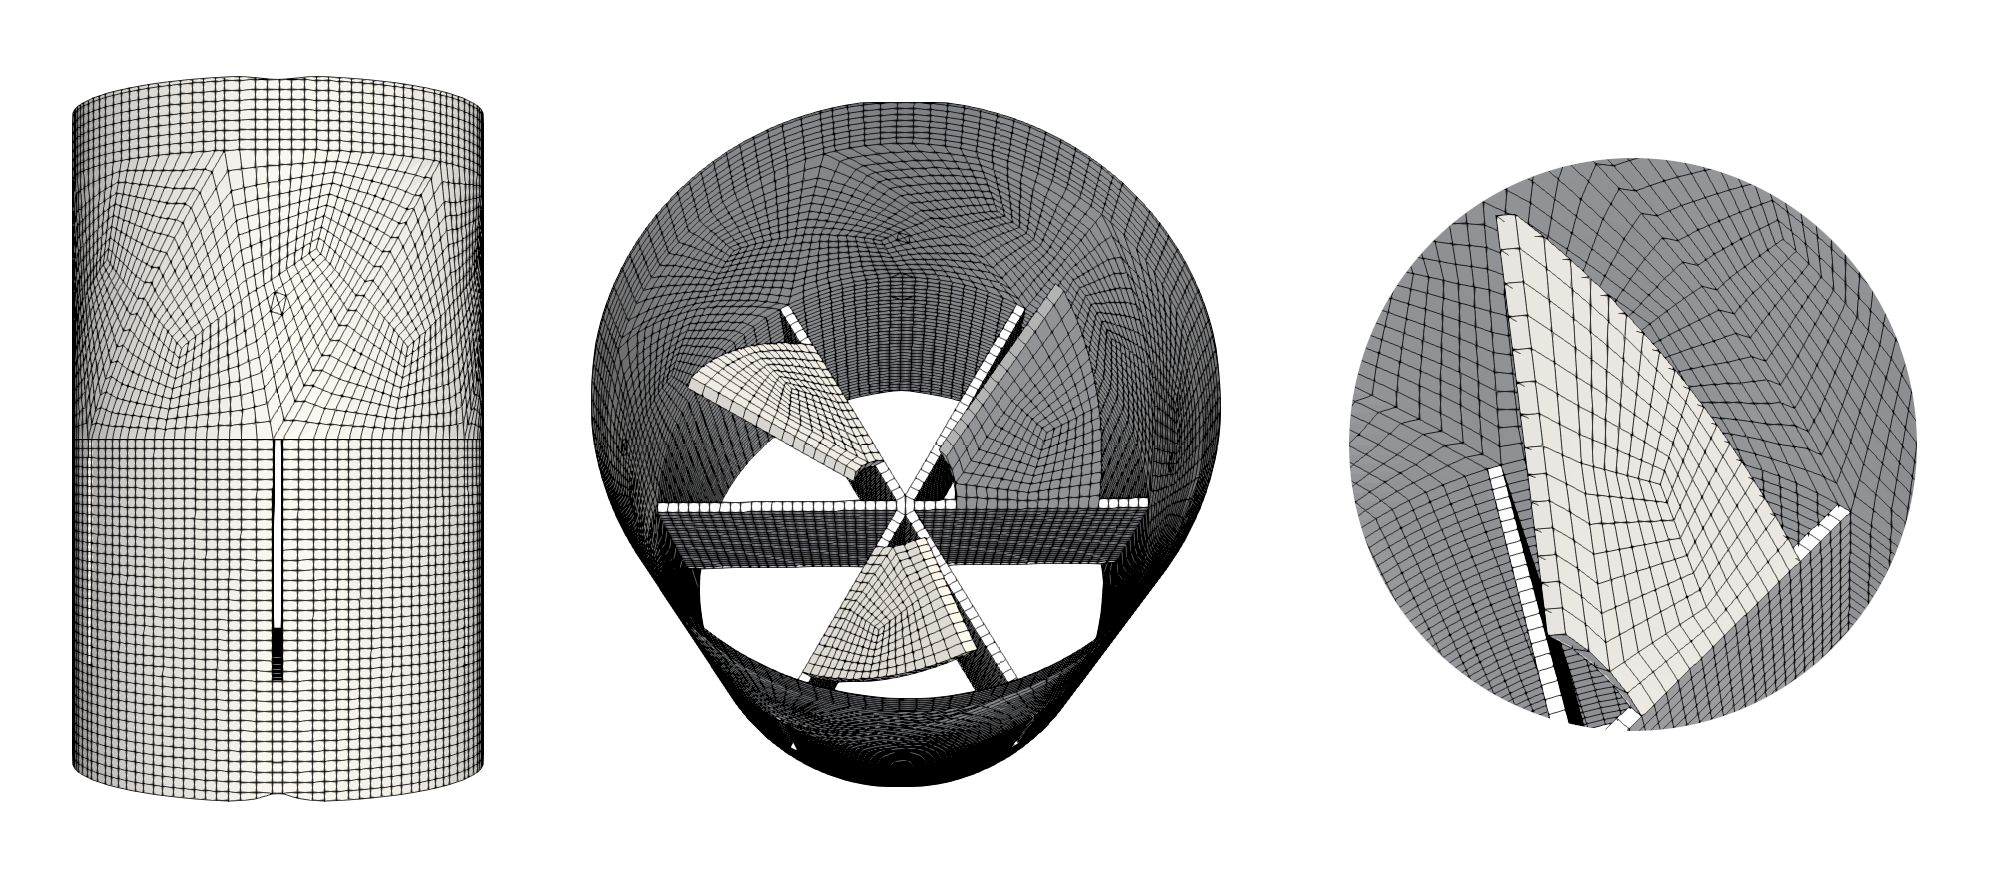
\includegraphics[width=1.0\linewidth]{img/DEBORA-Promoteur/cfd/prom_M2_all.png}
\caption{Meshing of the mixing vanes region.}
\label{fig:prom_M2}
\end{figure}
%

\npar


We simulated 3 cases per series 48G3P26WA and 52G3P26WA, covering the two MV positions and different outlet quality ($x_{eq,out}$) :

\begin{itemize}
\item 48G3P26WATe65 \& 52G3P26WATe65 with $x_{eq,out}\approx 0\%$ 
\item 48G3P26WATe69 \& 52G3P26WATe69 with $x_{eq,out}\approx 5\%$ 
\item 48G3P26WATe75 \& 52G3P26WATe75 with $x_{eq,out}\approx 12.5\%$ 
\end{itemize}

\begin{note*}{}
The computational times was ensured to be long enough to reach time-average convergence of the simulations.
\end{note*}


Results are compared to the experimental measurements \ie only void fraction for C4800 cases and void fraction, bubble diameter and vapor velocity for C5200 cases.

\begin{remark*}{}
Following the discussions regarding vapor velocity and bubble diameter estimation for C5200 cases (Chapter \ref{chap:debora_agate_prom}), comparison with the CFD results will rather be of qualitative nature since we can't ensure the accuracy of the measurements.
\end{remark*}


\subsection{Results}

Results are presented on Figure \ref{fig:debprom_ncfd}.

%
\begin{figure}[!htb]
\centering
\subfloat[Void fraction - Te65 cases]{
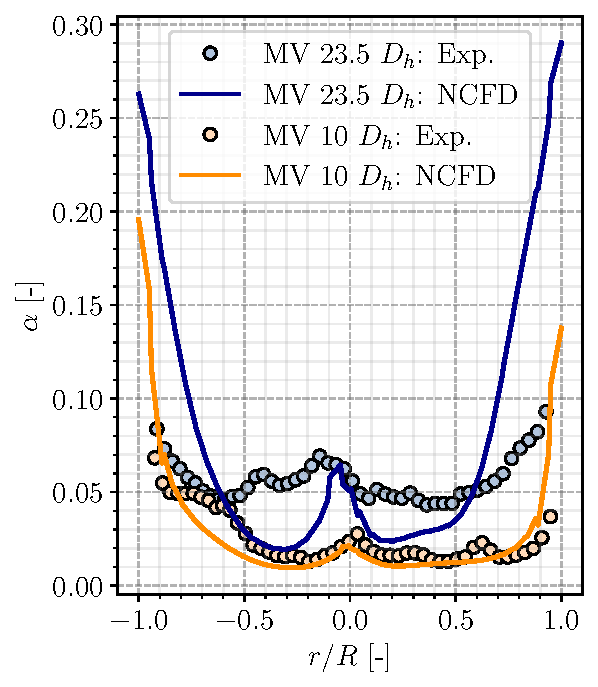
\includegraphics[width=0.33\linewidth]{img/DEBORA-Promoteur/cfd/G3P26W23Te65_alpha.pdf}
\label{fig:Te65_cfd_alpha}
}
\subfloat[Void fraction - Te69 cases]{
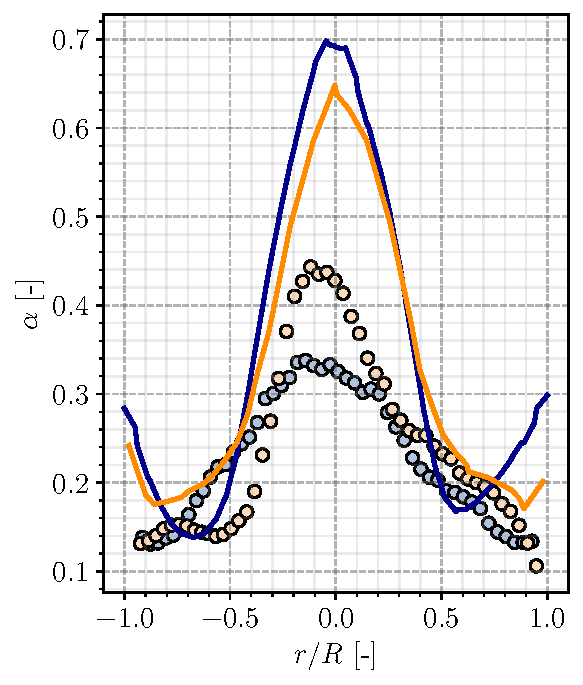
\includegraphics[width=0.33\linewidth]{img/DEBORA-Promoteur/cfd/G3P26W23Te69_alpha.pdf}
\label{fig:Te69_cfd_alpha}
}
\subfloat[Void fraction - Te75 cases]{
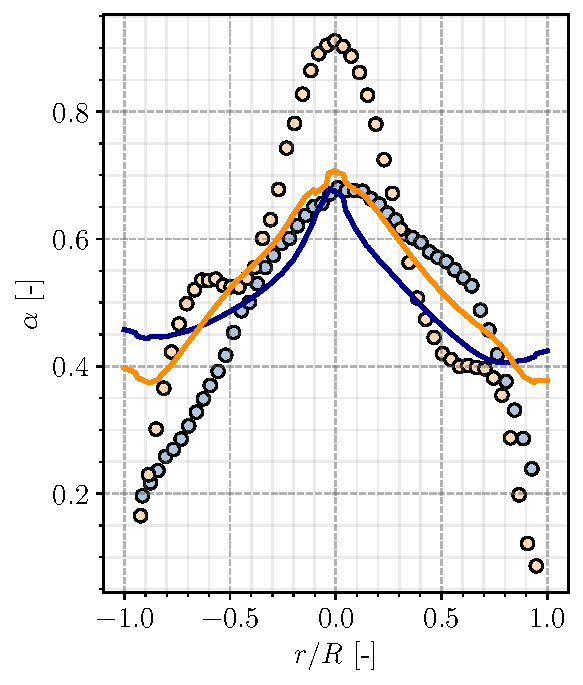
\includegraphics[width=0.33\linewidth]{img/DEBORA-Promoteur/cfd/G3P26W23Te75_alpha.pdf}
\label{fig:Te75_cfd_alpha}
}
\\
\subfloat[Bubble diameter - Te65 case]{
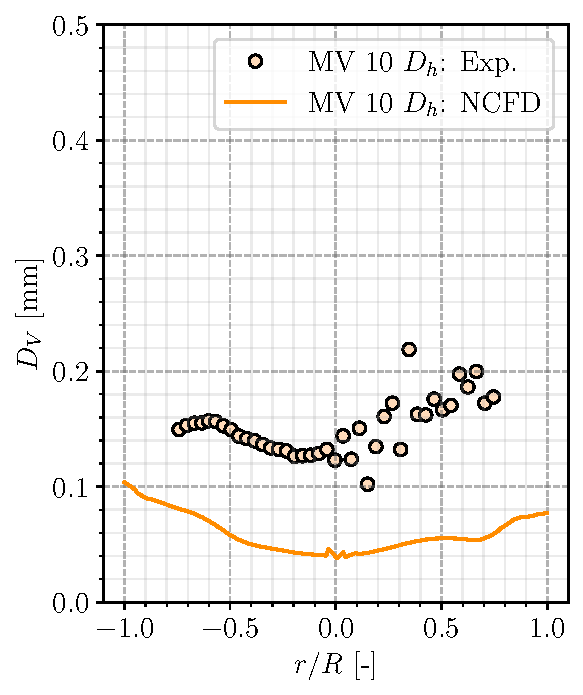
\includegraphics[width=0.33\linewidth]{img/DEBORA-Promoteur/cfd/G3P26W23Te65_dV.pdf}
\label{fig:Te65_cfd_dV}
}
\subfloat[Bubble diameter - Te69 case]{
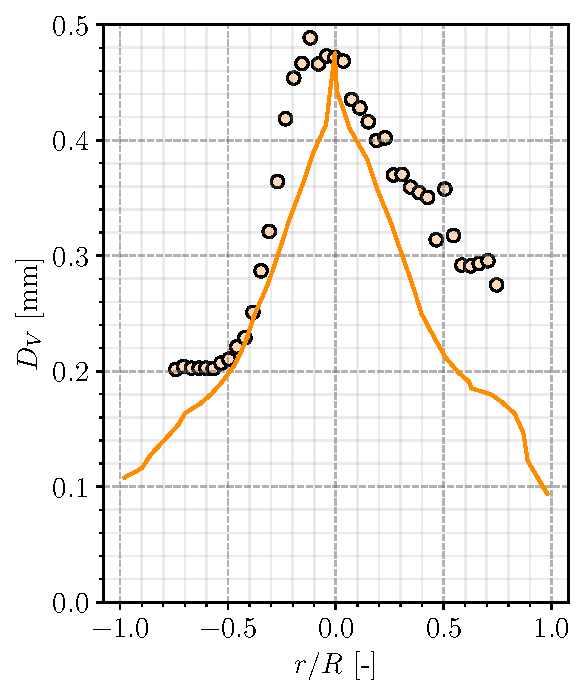
\includegraphics[width=0.33\linewidth]{img/DEBORA-Promoteur/cfd/G3P26W23Te69_dV.pdf}
\label{fig:Te69_cfd_dV}
}
\subfloat[Bubble diameter - Te75 case]{
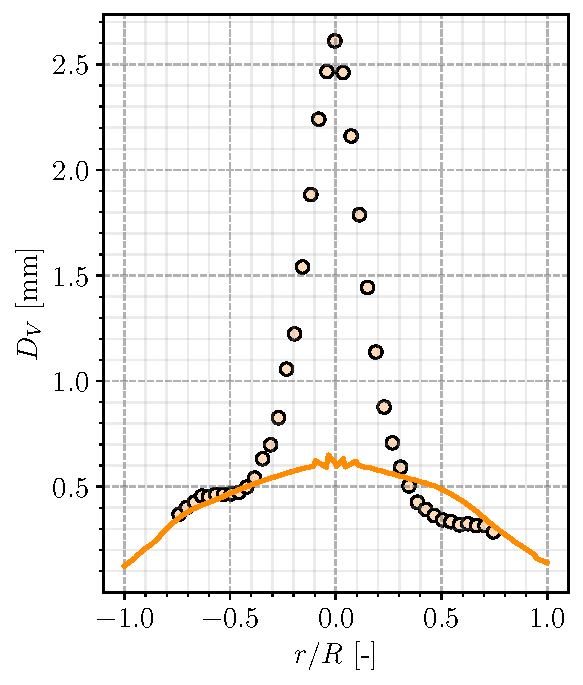
\includegraphics[width=0.33\linewidth]{img/DEBORA-Promoteur/cfd/G3P26W23Te75_dV.pdf}
\label{fig:Te75_cfd_dV}
}
\\
\subfloat[Vapor axial velocity - Te65 case]{
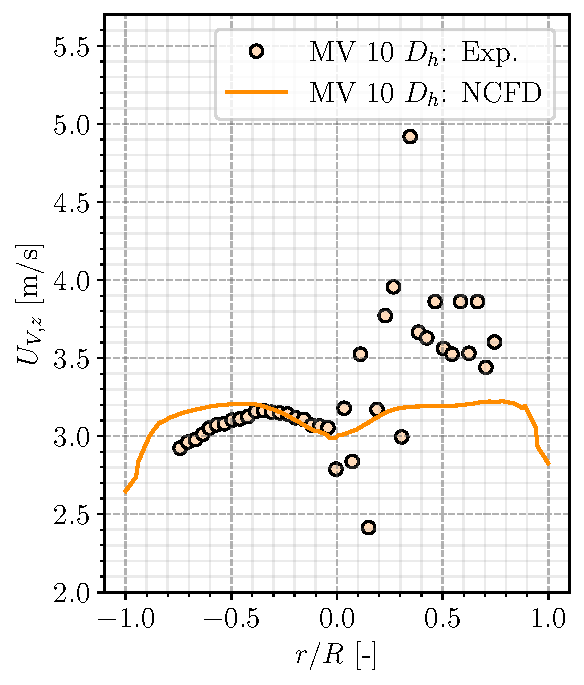
\includegraphics[width=0.33\linewidth]{img/DEBORA-Promoteur/cfd/G3P26W23Te65_Uvap.pdf}
\label{fig:Te65_cfd_Uvap}
}
\subfloat[Vapor axial velocity - Te69 case]{
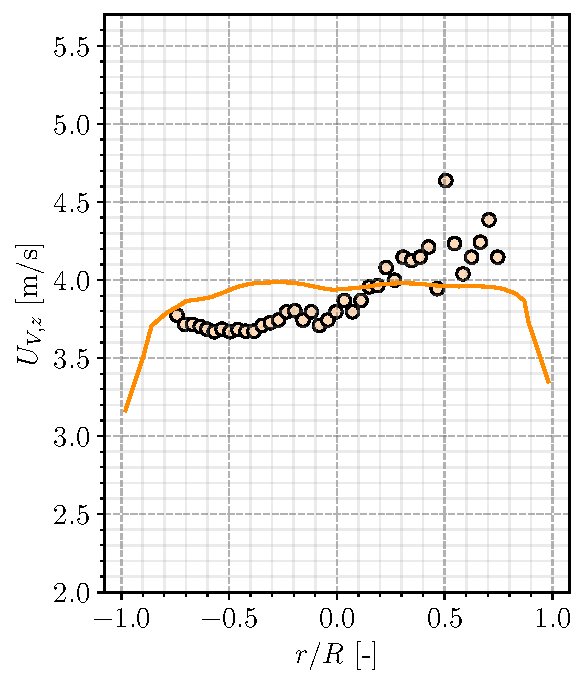
\includegraphics[width=0.33\linewidth]{img/DEBORA-Promoteur/cfd/G3P26W23Te69_Uvap.pdf}
\label{fig:Te69_cfd_Uvap}
}
\subfloat[Vapor axial velocity - Te75 case]{
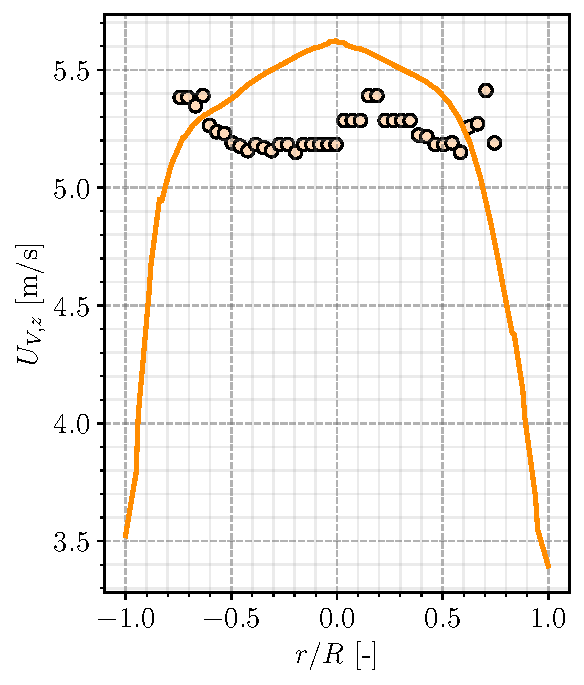
\includegraphics[width=0.33\linewidth]{img/DEBORA-Promoteur/cfd/G3P26W23Te75_Uvap.pdf}
\label{fig:Te75_cfd_Uvap}
}
\caption{NCFD results on the DEBORA-Promoteur cases. MV at $23.5\ D_{h}$ and $10\ D_{h}$respectively correspond to C4800 and C5200 cases.}
\label{fig:debprom_ncfd}
\end{figure}
%



\clearpage



Quantitatively speaking, it seems that NEPTUNE\_CFD reproduces the effect of vapor accumulation at the center under the pressure gradient generated by the swirl induced by the mixing vanes. The radial position of the core void fraction peak correctly matches the experimental one. The Te65 cases (Figure \ref{fig:Te65_cfd_alpha}) are reasonably predicted with void fractions values at the center close to the measurements, with the C5200 simulation much closer to the experimental profile. However, Te69 and Te75 cases (Figures \ref{fig:Te69_cfd_alpha} and \ref{fig:Te75_cfd_alpha}) are showing much larger discrepancies with the experiments. The core void fraction peak appears largely overestimated for $T_{L,in}=69\degC$ with $\alpha\parth{r/R= 0} \approx 70\%$ and do not change when moving to $T_{L,in}=75\degC$ where the void fraction profile rather flattens. Such a behavior strongly differs from the experiments where a large increase in core void fraction when inlet temperature increases. Moreover, the particular shape of 52G3P26WATe75 case where local maximum for $\alpha$ are observed at $r/R \approx \pm 0.6$.

\begin{remark*}{}
The computed void fraction seems unable to go above 70\% in this case, which is in contradiction with the experiments. However, a sensitivity test showed that removing all the interfacial forces except the drag (Eq. \ref{eq:ncfd_drag}) allowed the bulk void fraction to reach $90\%$ as presented on Figure \ref{fig:prom_onlydrag}.

\end{remark*}

\begin{figure}[!h]
\centering
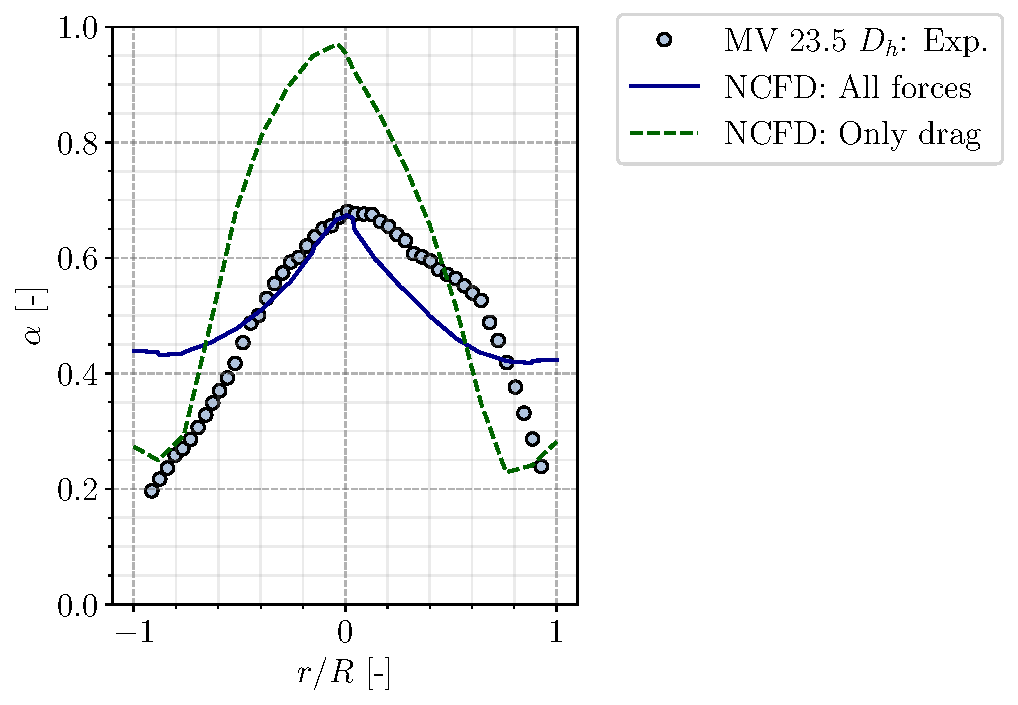
\includegraphics[width=0.5\linewidth]{img/DEBORA-Promoteur/cfd/G3P26W23Te75_alpha_drag.pdf}
\caption{Sensitivity test on case 48G3P26WATe75 leaving only the drag force in the interfacial momentum closure.}
\label{fig:prom_onlydrag}
\end{figure}


\npar

Regarding C5200 cases, bubble diameter profiles appear coherent with the experimental estimations for Te65 and Te69 cases (Figure \ref{fig:Te65_cfd_dV} and \ref{fig:Te69_cfd_dV}). In particular, the growth towards the center due to coalescence is fairly reproduced in Te69 case. On the contrary, the very large estimated values for Te75 case ($D_{V} \sim 2\ $mm) are completely missed by the simulation (Figure \ref{fig:Te75_cfd_dV}).

\begin{remark*}{}
As discussed in the analysis of the experimental results (Subsection \ref{subsec:debprom_dV_exp}), the flow regime encountered in the 52G3P26W3Te75 case is very likely deviate from a dispersed flow (very large void fractions), explaining the inability of the simulations to reproduce this behavior.
\end{remark*}


\npar


Finally, the order of magnitude of predicted vapor velocities increases with the inlet temperature (Figures \ref{fig:Te65_cfd_Uvap}, \ref{fig:Te69_cfd_Uvap}, \ref{fig:Te75_cfd_Uvap}) similarly to the experimental estimations.

\npar


To further investigate the mixing vanes geometry and understand the large discrepancies on the void fraction profiles (Figures \ref{fig:Te69_cfd_alpha} and \ref{fig:Te75_cfd_alpha}), we perform simulations of the single-phase AGATE-Promoteur case in next Section.





\section{NEPTUNE\_CFD simulations of AGATE-Promoteur cases}
\label{sec:agate_ncfd}


\subsection{Simulation Setup}

Simulations of the AGATE-Promoteur case are done using \textit{code\_saturne} 7.0, the single-phase counterpart of NEPTUNE\_CFD. The computational domain is 0.7\ m long (shorter than DEBORA-Promoteur case since we don't need to apply the 3.5m heating) with the mixing blades positioned at $z=0$. Using the same meshing used for the DEBORA-Promoteur cases (Figure \ref{fig:prom_M2}), the total mesh contains 1~905~357 cells.

\npar

Two simulations are performed using the turbulence model $R_{ij}-\varepsilon$ SSG with a smooth wall two-scale turbulent law and with a rough wall turbulent law (average roughness $\epsilon = 10^{-5}$\ m fixed arbitrarily as a sensitivity test). The usual wall law in \textit{code\_saturne} is a two friction velocity scales law \cite{noauthor_code_saturne_2021}, with the roughness inducing a shift in the logarithmic term of the non-dimensional velocity:

\begin{equation}
u^{+} = \frac{1}{\kappa}\ln{\dfrac{y+\epsilon}{\epsilon}} + C_{log}
\end{equation}
with $C_{log}=5.2$ and $y$ the absolute distance to the wall.



\npar
\begin{note*}{}
Before comparisons with experiments, we made sure that NEPTUNE\_CFD two-phase solver and \textit{code\_saturne} single-phase solver produced similar results when simulating a single-phase flow using the $R_{ij}-\varepsilon$ SSG model.
\end{note*}

\npar


To test the sensitivity to turbulence modeling, we also realize a Large Eddy Simulation (LES) using the LES WALE (Wall-Adapting Local Eddy-Viscosity) model \cite{nicoud_subgrid-scale_1999}. For this simulation, we use a more refined mesh (Figure \ref{fig:prom_M4}) containing a total of 121~942~848 cells. 

%
\begin{figure}[!h]
\centering
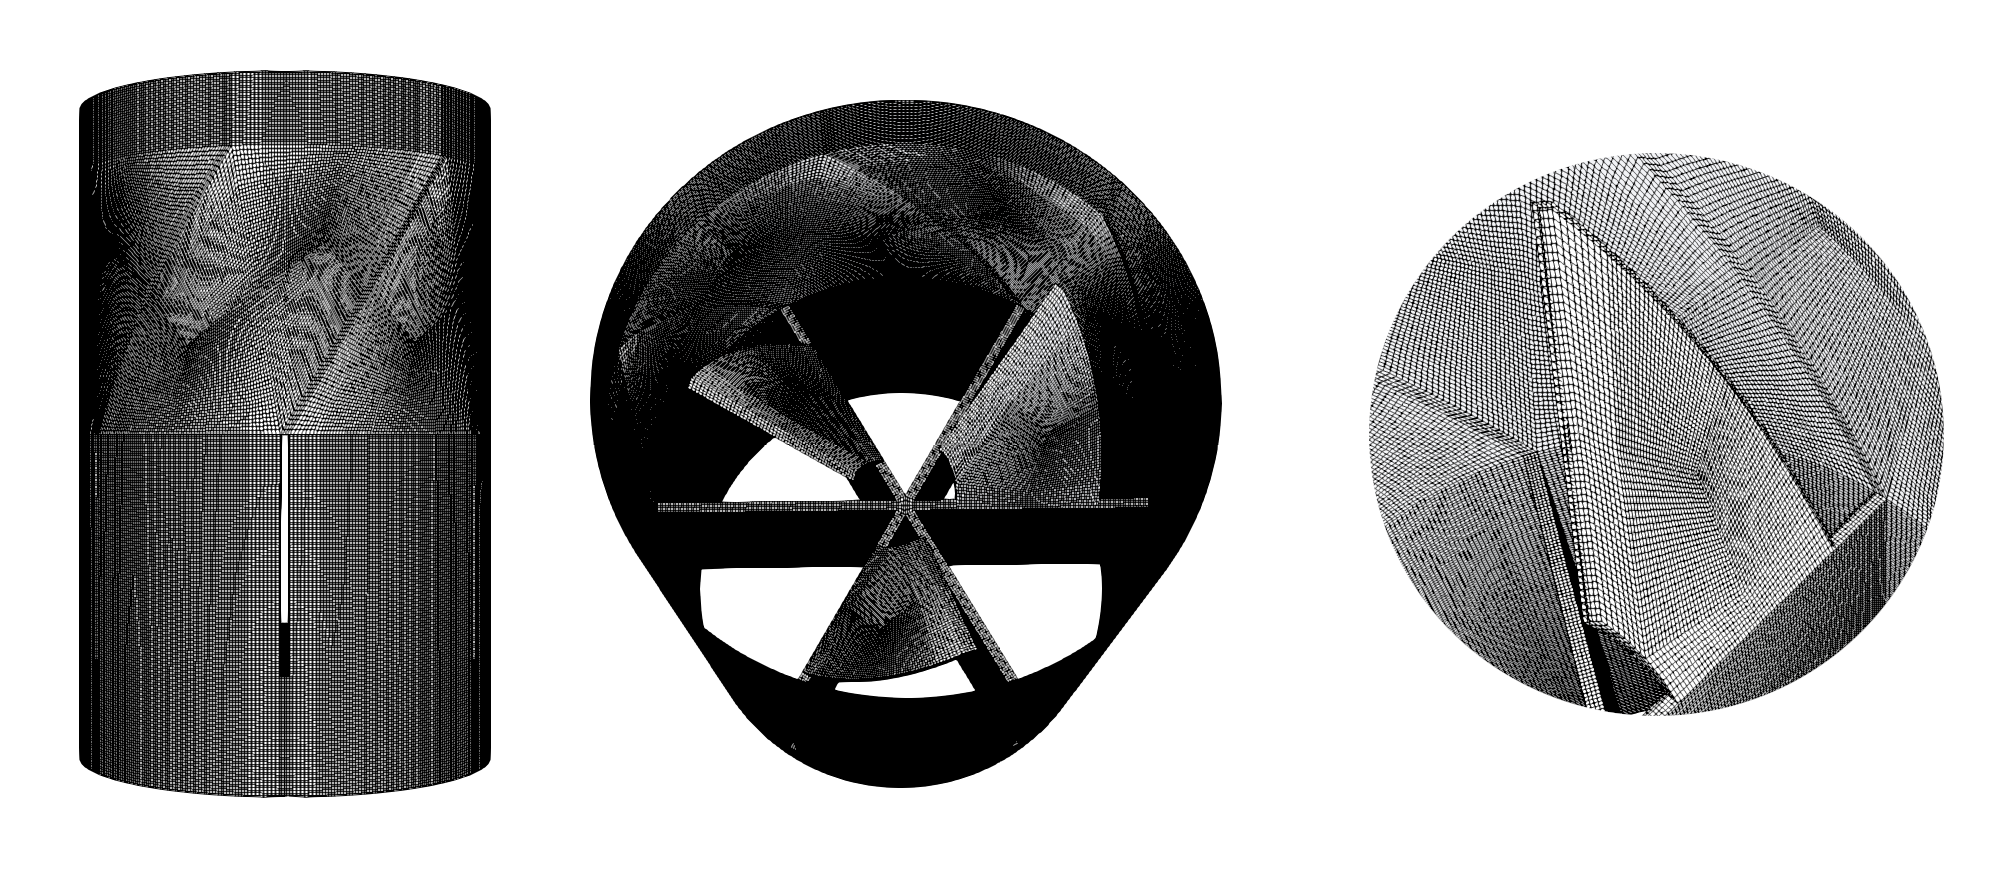
\includegraphics[width=1.0\linewidth]{img/AGATE/prom_M4_all.png}
\caption{Fine meshing of the mixing vanes region for the LES calculation.}
\label{fig:prom_M4}
\end{figure}
%

\npar


In this configuration, we achieve an average wall distance $y^{+} \approx 13$ in the whole domain (while $y^{+} \approx 50$ for the other mesh), which is too large to numerically resolve the boundary layer meaning a wall-law will be used to evaluate the liquid velocity in the wall cell. 

\begin{note*}{}
A stable time-convergence of all the variables is achieved for the LES computation after 10~s of simulated physical time.
\end{note*}

\npar

Finally, we want to compare the results of the simulations with measurements of the RMS of the velocity fluctuations (Eq. \ref{eq:RMS_def}), meaning that we have to reconstruct those values from the CFD computations. Since we perform Unsteady-RANS (URANS) simulations (using the $R_{ij}-\varepsilon$ SSG model), fluctuations of the velocity field are both modeled in the components of the Reynolds Stress Tensor and partly simulated due to the potential time-oscillations of the average velocity field $\left<\vect{U}\right>$. Therefore, the RMS for URANS simulations is computed using the modeled components of the Reynolds Stress Tensor $R_{ij,mod}$:

\begin{equation}
RMS_{A,URANS} = \sqrt{R_{zz,mod} + \left< \left(\tilde{U} \otimes \tilde{U}\right)_{zz}\right>}
\label{eq:RMS_URANS}
\end{equation}
where $\tilde{U} = \left<\vect{U}\right> - \vect{U}$ is the instantaneous difference between the velocity field and its time average \ie the simulated fluctuations of the URANS computation.

\npar

Regarding the LES computation, the fluctuations of the velocity field are mainly simulated and are thus only contained in the instantaneous velocity field $\vect{U}$. Therefore, they are computed as:

\begin{equation}
RMS_{A,LES} = \sqrt{\left< \left(\tilde{U} \otimes \tilde{U}\right)_{zz} \right>}
\label{eq:RMS_LES}
\end{equation}

\npar

The same operation is conducted for the radial RMS, which involves the components ${xx}$, ${yy}$ and ${xy}$.



\subsection{Results}

In this section, we discuss results obtained at three different heights : $0.8\ D_{h}$, $10\ D_{h}$ and $23\ D_{h}$ downstream the mixing vanes.


\subsubsection{$0.8\ D_{h}$ After the Mixing Vanes}

Figure \ref{fig:agate_cfd_1dh} shows the results less than a hydraulic diameter after the mixing vanes. As mentioned in previous Section, a sensitivity to the wall modeling is realized by performing an extra simulation including a wall roughness.


\begin{figure}[!h]
\centering
\subfloat[Axial velocity]{
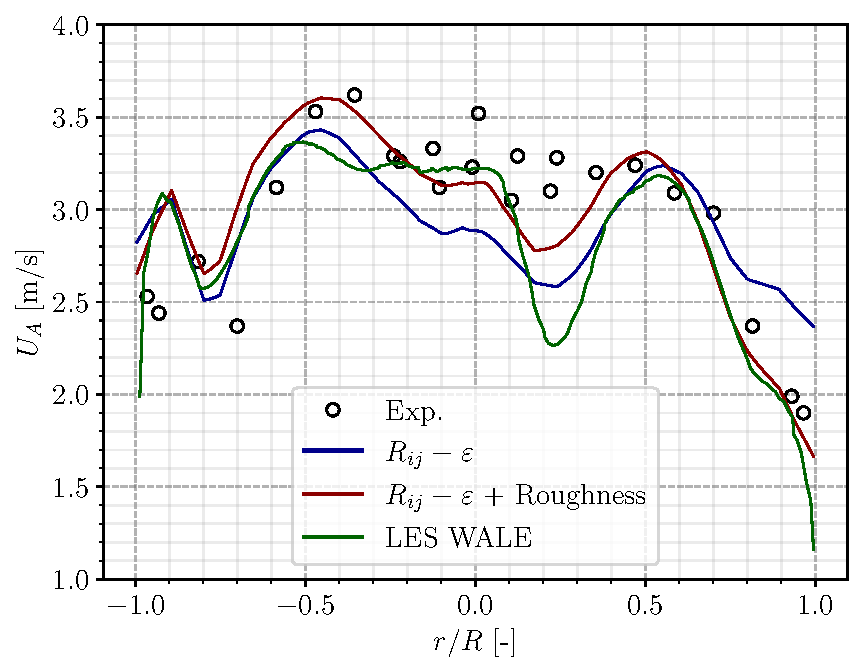
\includegraphics[width=0.4\linewidth]{img/AGATE/z15/pos1112_VA.pdf}
\label{fig:agate_1dh_UA}
}
\subfloat[Radial velocity]{
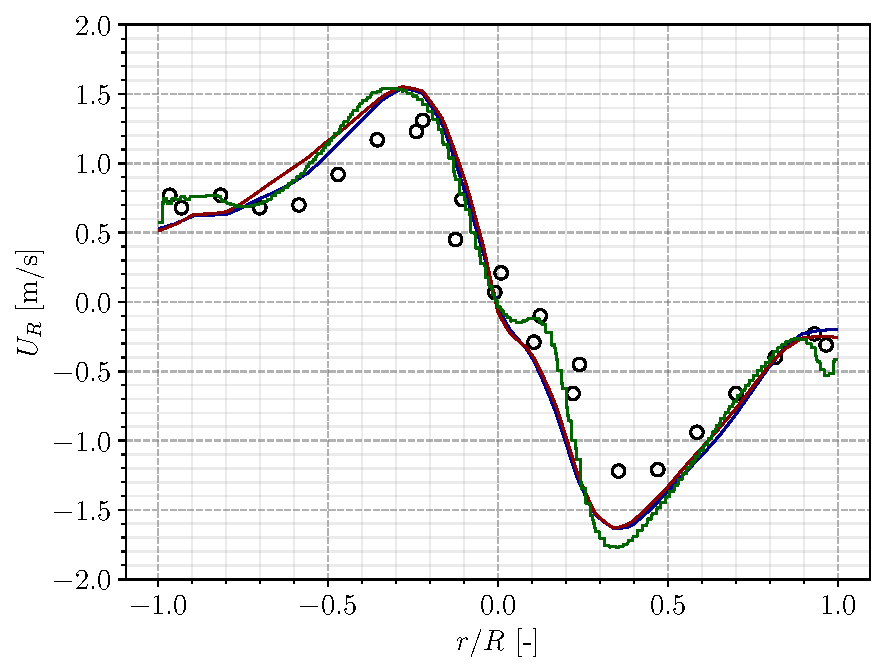
\includegraphics[width=0.4\linewidth]{img/AGATE/z15/pos1112_VT.pdf}
\label{fig:agate_1dh_UR}
}
\\
\subfloat[Axial RMS]{
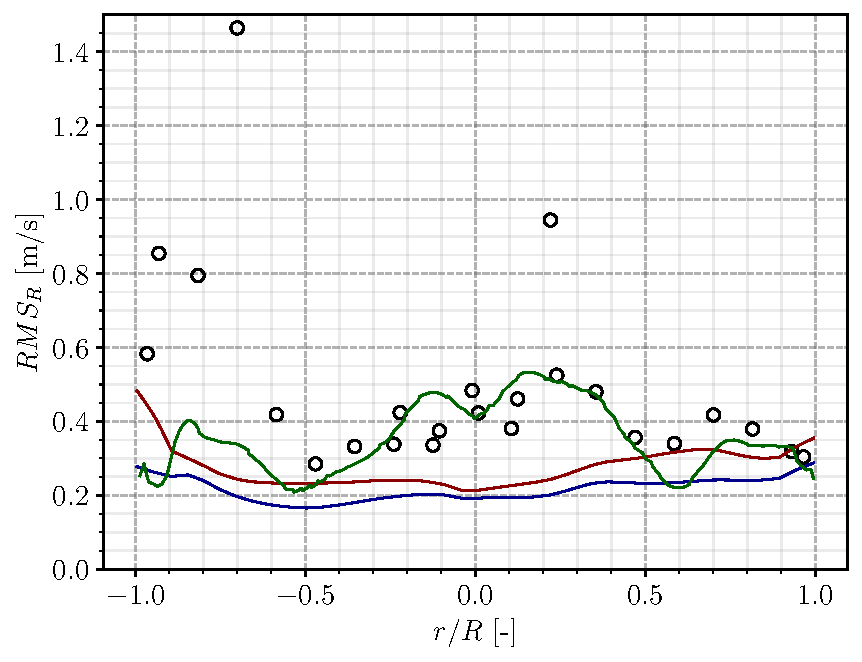
\includegraphics[width=0.4\linewidth]{img/AGATE/z15/pos1112_RMS_A.pdf}
\label{fig:agate_1dh_RMSA}
}
\subfloat[Radial RMS]{
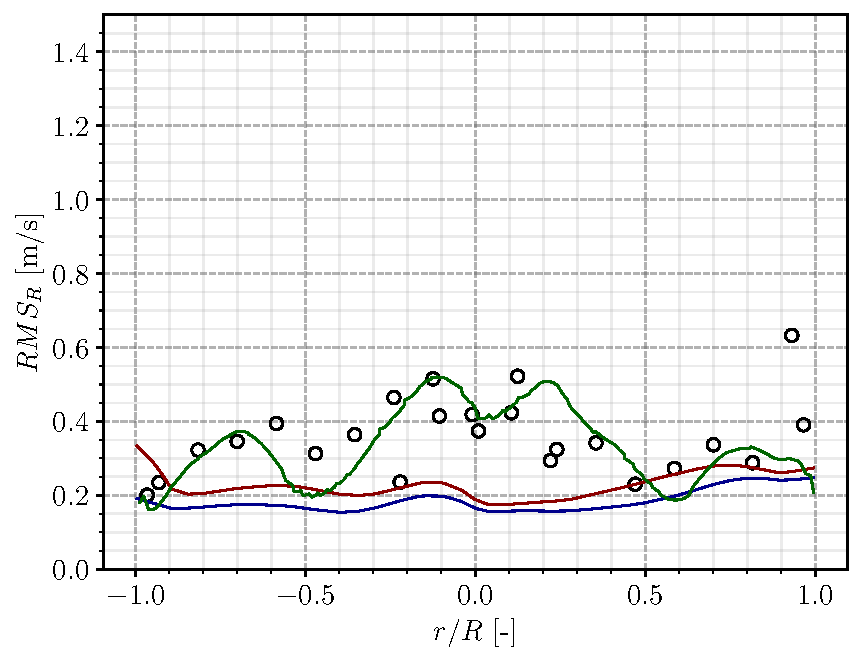
\includegraphics[width=0.4\linewidth]{img/AGATE/z15/pos1112_RMS_T.pdf}
\label{fig:agate_1dh_RMSR}
}
\caption{Results for $z=0.8\ D_{h}$}
\label{fig:agate_cfd_1dh}
\end{figure}

\npar


The three simulations correctly match the experiments for the axial and radial velocities (Figures \ref{fig:agate_1dh_UA} and \ref{fig:agate_1dh_UR}). However, the velocity RMS (Figures \ref{fig:agate_1dh_RMSA} and \ref{fig:agate_1dh_RMSR}) are underestimated by the $R_{ij}-\varepsilon$ model, with the rough law use yielding slightly higher values. On the contrary, the LES simulation better reproduce the core velocity fluctuations especially near the center of the pipe.


\npar

Figure \ref{fig:ur_s_ua_1dh} shows the ratio of radial to axial velocity $1~D_{h}$ after the vanes for the LES computation.

\begin{figure}
\subfloat[Instantaneous values]{
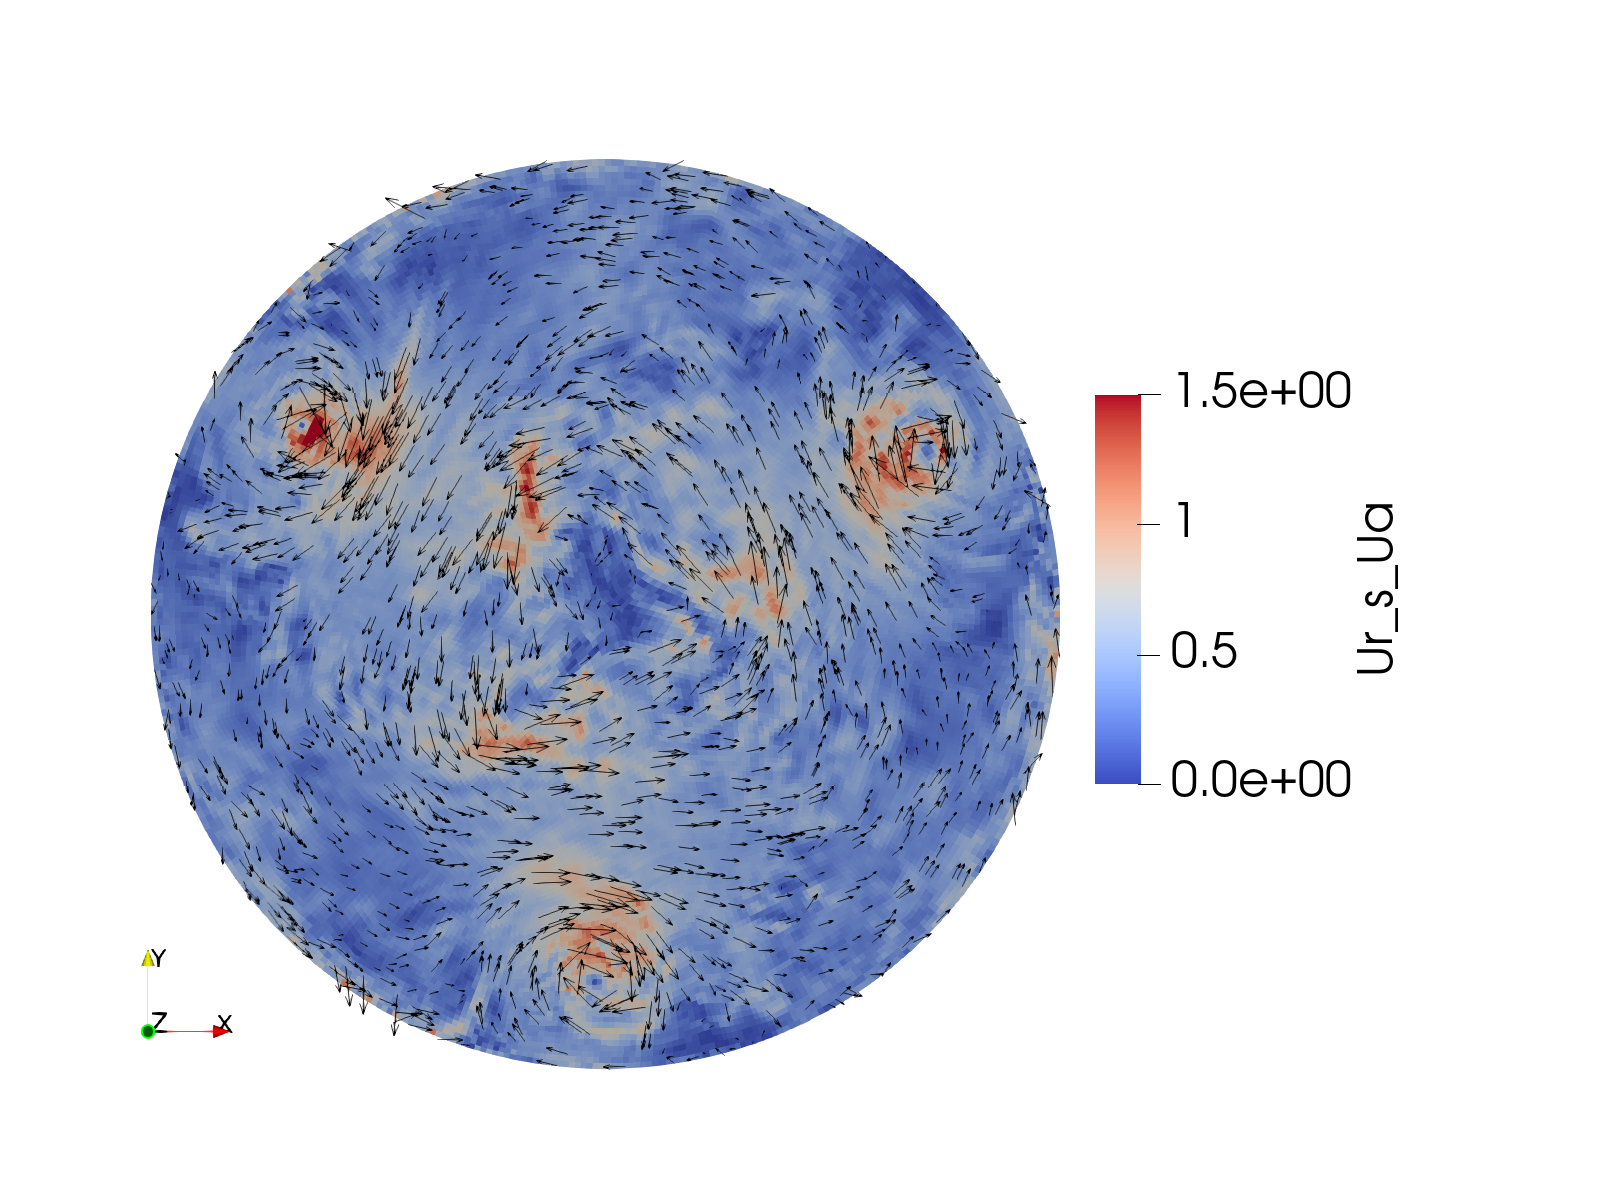
\includegraphics[width=0.5\linewidth]{img/AGATE/Ur_s_Ua/1Dh_Ur_s_Ua.png}
}
\subfloat[Time-averaged values]{
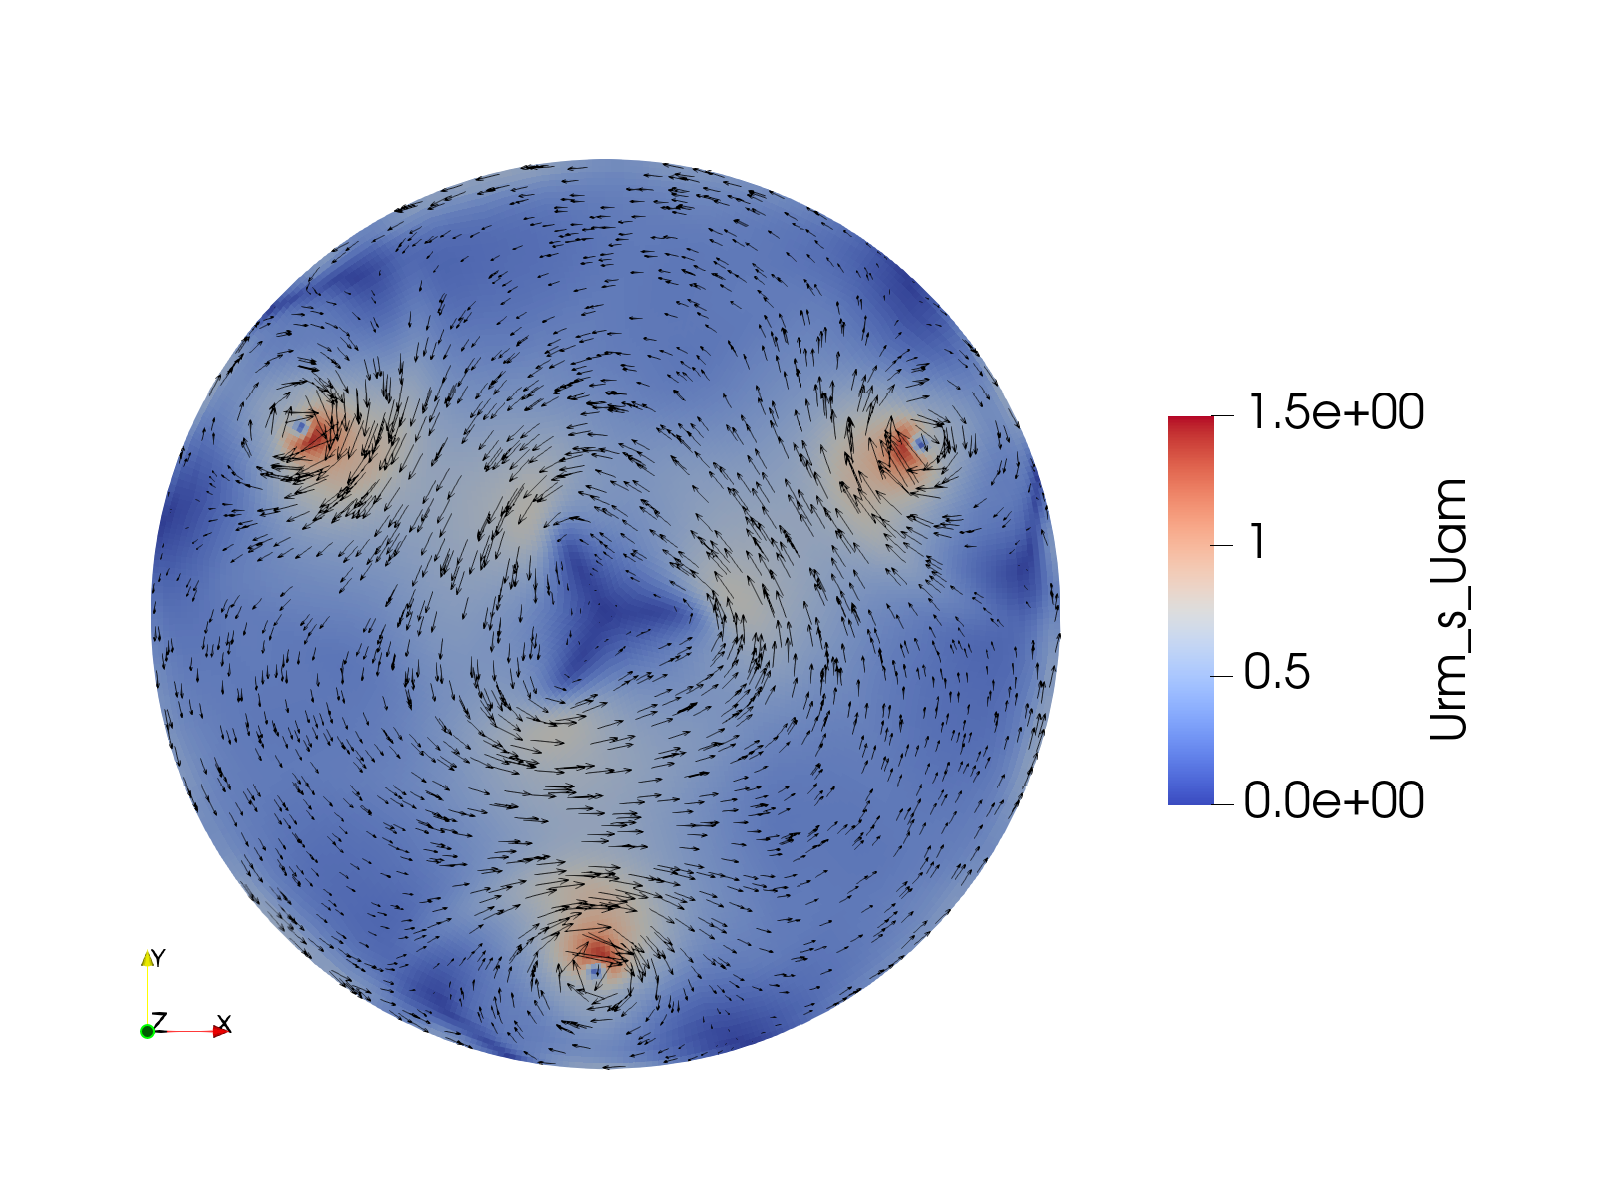
\includegraphics[width=0.5\linewidth]{img/AGATE/Ur_s_Ua/1Dh_Urm_s_Uam.png}
}
\caption{Visualization of the radial velocity field and ratio between radial and axial velocity obtained with the LES, $z=1~D_{h}$ downstream the MV.}
\label{fig:ur_s_ua_1dh}
\end{figure}



\npar


\subsubsection{$10\ D_{h}$ After the Mixing Vanes}

Figure \ref{fig:agate_cfd_10dh} shows the results at $10\ D_{h}$ downstream the mixing vanes, which corresponds to the distance at which two-phase flow measurements of the DEBORA-Promoteur C5200 campaign was conducted (Section \ref{sec:deb_prom_desc}.

\begin{figure}[!h]
\centering
\subfloat[Axial velocity]{
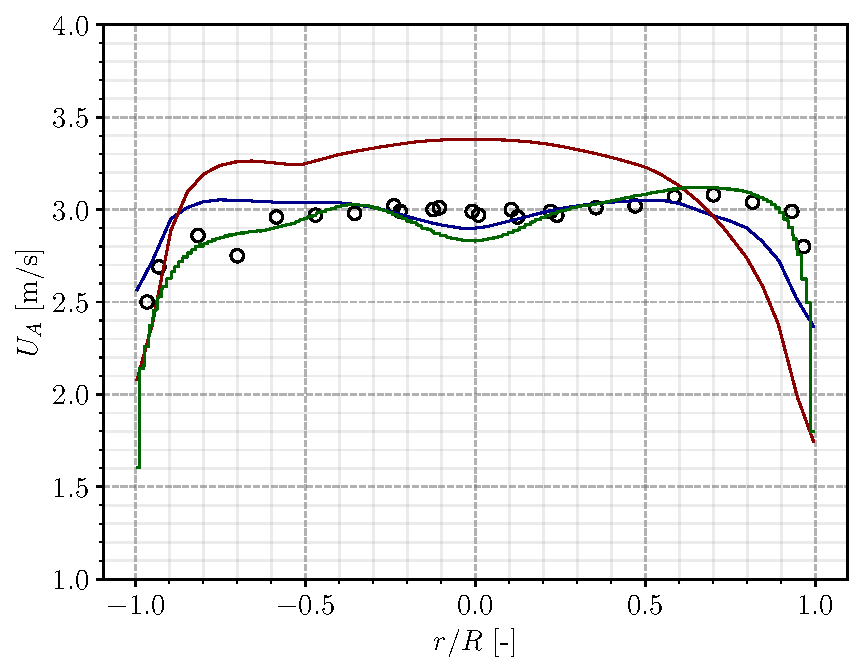
\includegraphics[width=0.4\linewidth]{img/AGATE/z200/pos910_VA.pdf}
\label{fig:agate_10dh_UA}
}
\subfloat[Radial velocity]{
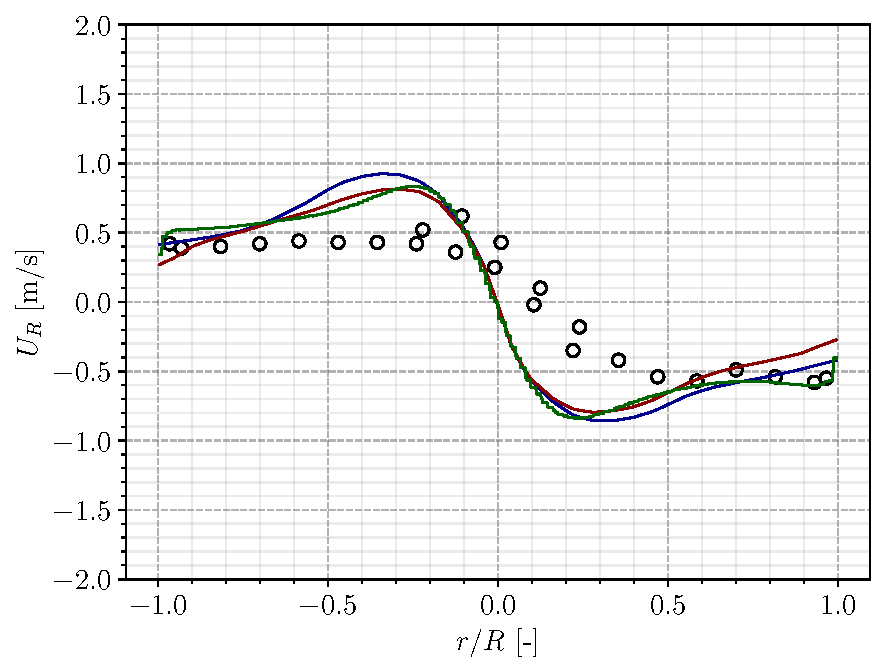
\includegraphics[width=0.4\linewidth]{img/AGATE/z200/pos910_VT.pdf}
\label{fig:agate_10dh_UR}
}
\\
\subfloat[Axial RMS]{
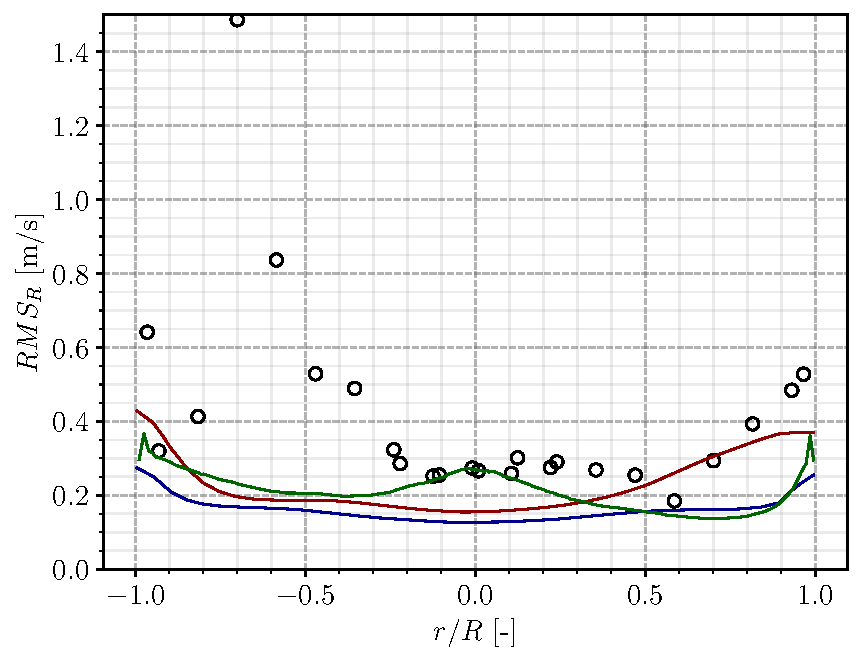
\includegraphics[width=0.4\linewidth]{img/AGATE/z200/pos910_RMS_A.pdf}
\label{fig:agate_10dh_RMSA}
}
\subfloat[Radial RMS]{
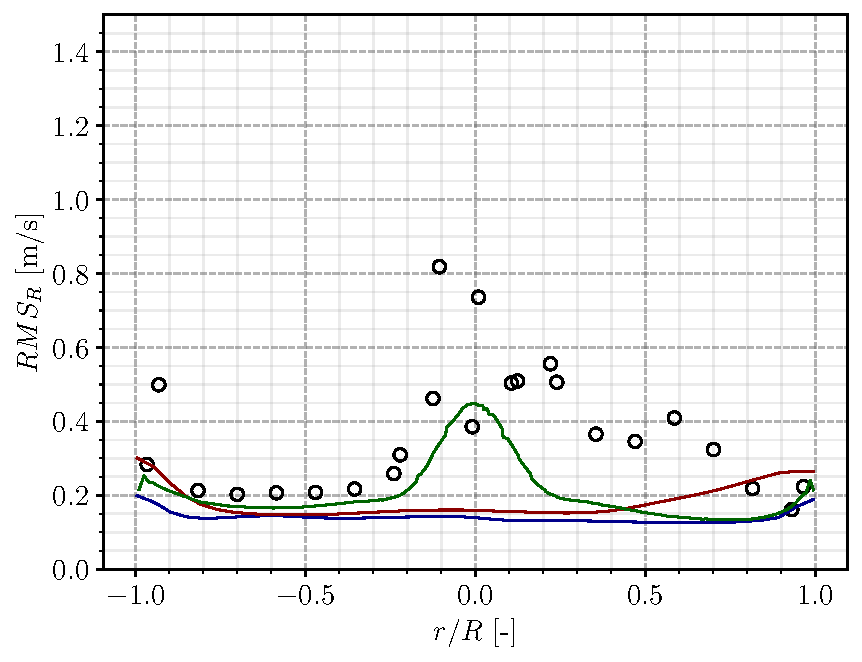
\includegraphics[width=0.4\linewidth]{img/AGATE/z200/pos910_RMS_T.pdf}
\label{fig:agate_10dh_RMSR}
}
\caption{Results for $z=10.4\ D_{h}$}
\label{fig:agate_cfd_10dh}
\end{figure}

Going further downstream, we observe that the use of the roughness law start to induce discrepancies on the axial velocity profile while the two other calculations still agree with the measurements (Figure \ref{fig:agate_10dh_UA}). Radial velocity is however equally predicted by the three simulations, with well reproduced wall values but all showing overestimation for $-0.5 \leq r/R \leq 0.5$ (Figure \ref{fig:agate_10dh_UR}), meaning that a too large bulk rotation of the fluid is predicted. 

\npar

The velocity RMS are still better predicted by the LES computation (Figures \ref{fig:agate_10dh_RMSA} and \ref{fig:agate_10dh_RMSR}) but start to show underprediction compared to the $1\ D_{h}$ results. Close to the wall, the three modeling all perform similarly.


\npar

Figure \ref{fig:ur_s_ua_10dh} shows the ratio of radial to axial velocity $10~D_{h}$ after the vanes for the LES computation.

\begin{figure}
\subfloat[Instantaneous values]{
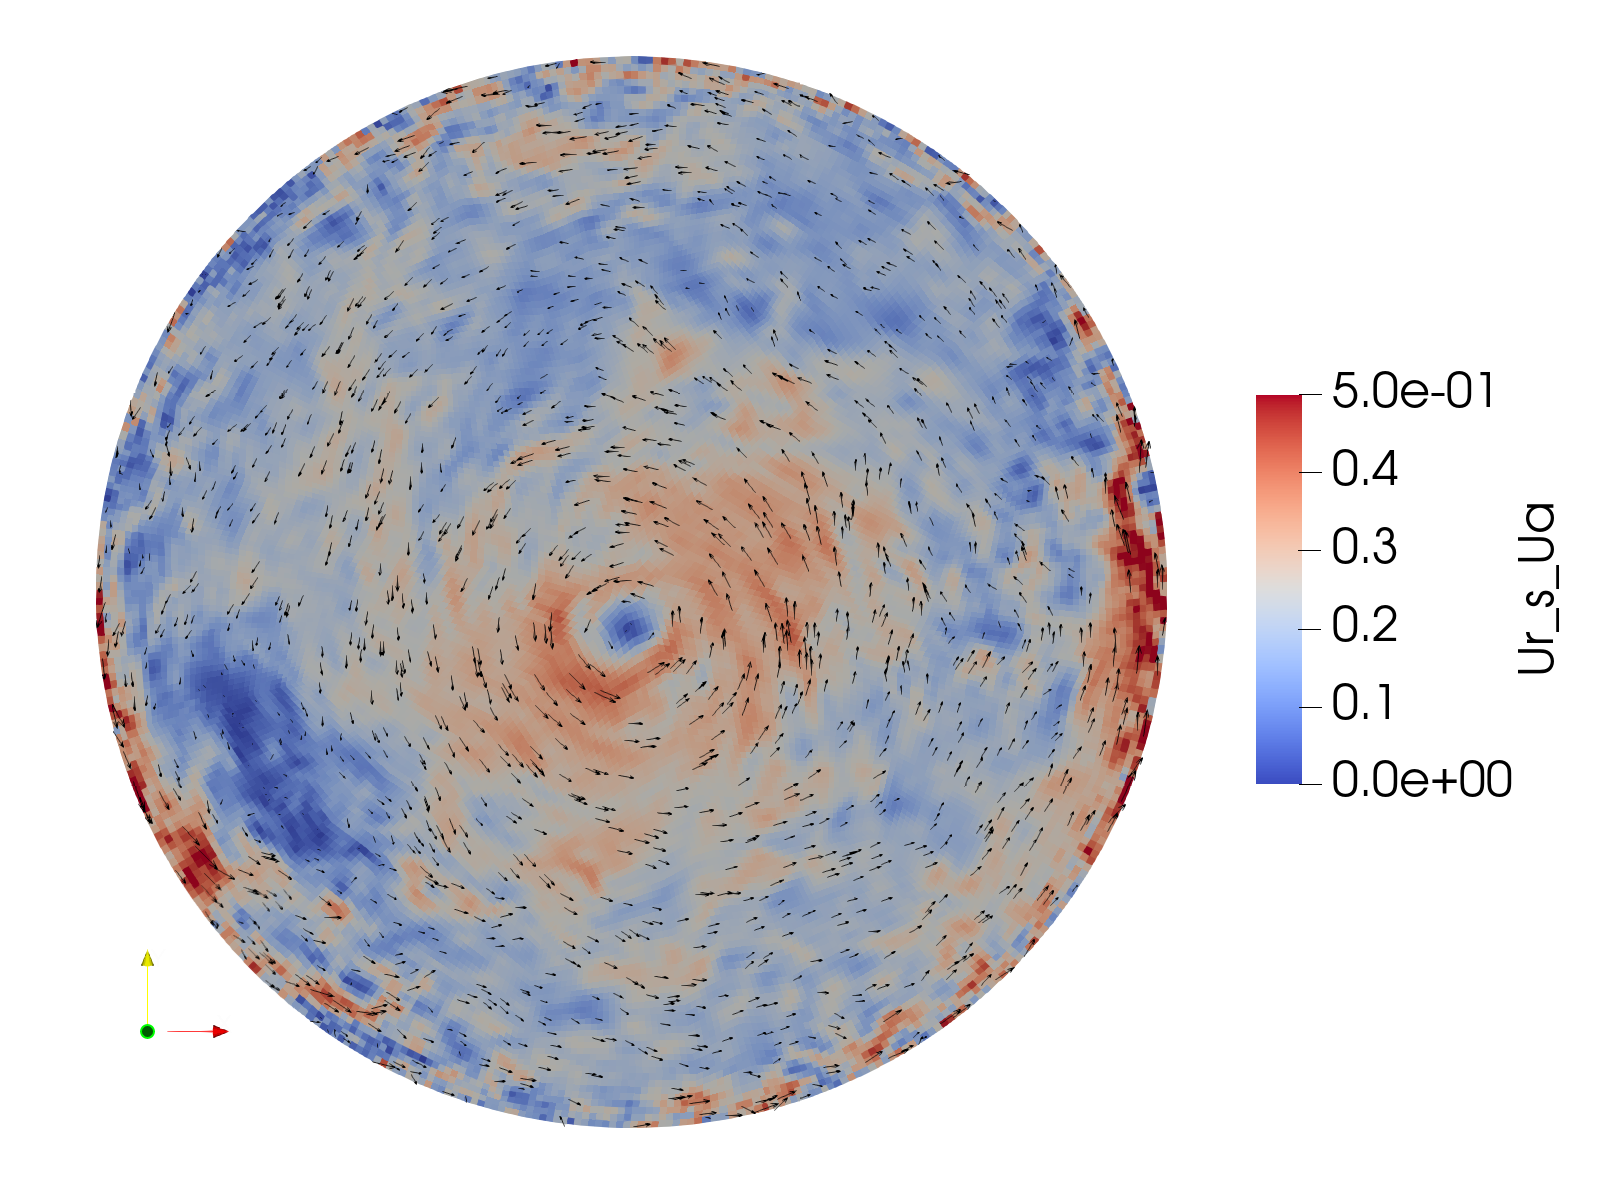
\includegraphics[width=0.5\linewidth]{img/AGATE/Ur_s_Ua/10Dh_Ur_s_Ua.png}
}
\subfloat[Time-averaged values]{
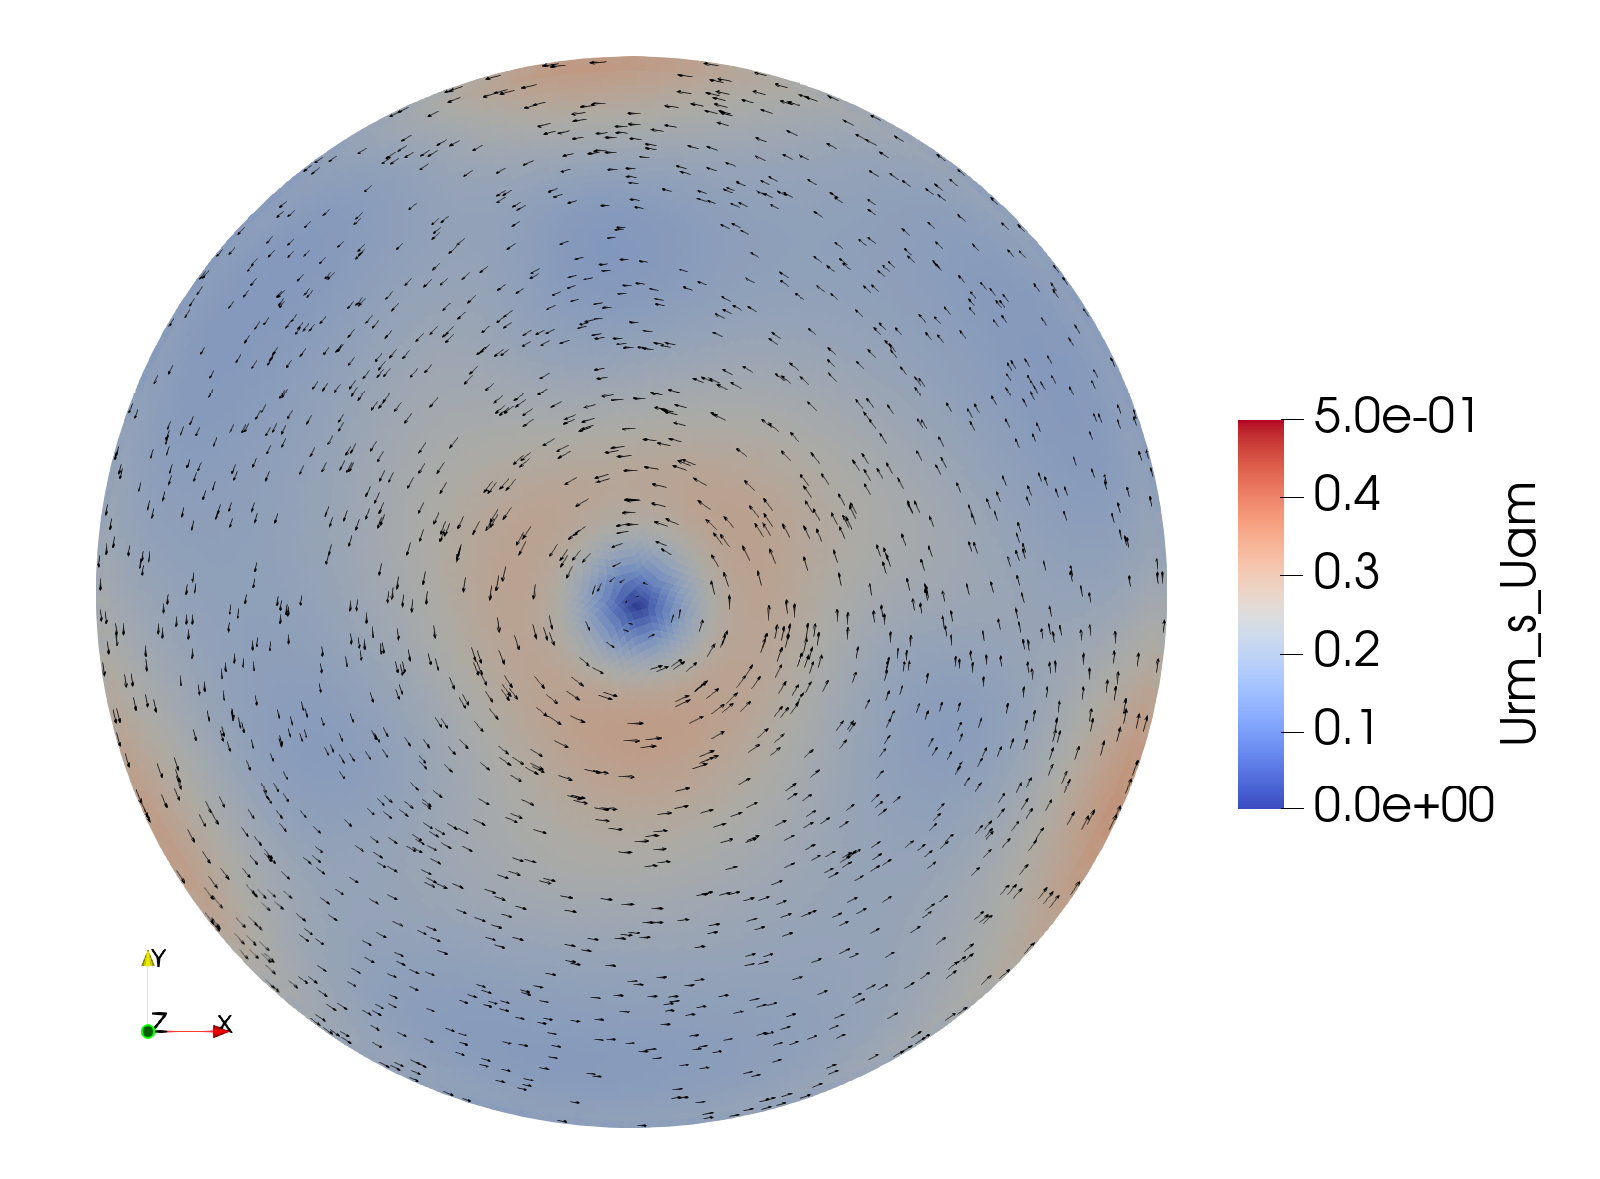
\includegraphics[width=0.5\linewidth]{img/AGATE/Ur_s_Ua/10Dh_Urm_s_Uam.png}
}
\caption{Visualization of the radial velocity field and ratio between radial and axial velocity obtained with the LES, $z=10~D_{h}$ downstream the MV.}
\label{fig:ur_s_ua_10dh}
\end{figure}



\npar


\subsubsection{$23\ D_{h}$ After the Mixing Vanes}

Finally, Figure \ref{fig:agate_cfd_23dh} present results $23.5\ D_{h}$ downstream the mixing vanes, which corresponds to the distance at which two-phase flow measurements of the DEBORA-Promoteur C4800 campaign was conducted (Section \ref{sec:deb_prom_desc}.


\begin{figure}[!h]
\centering
\subfloat[Axial velocity]{
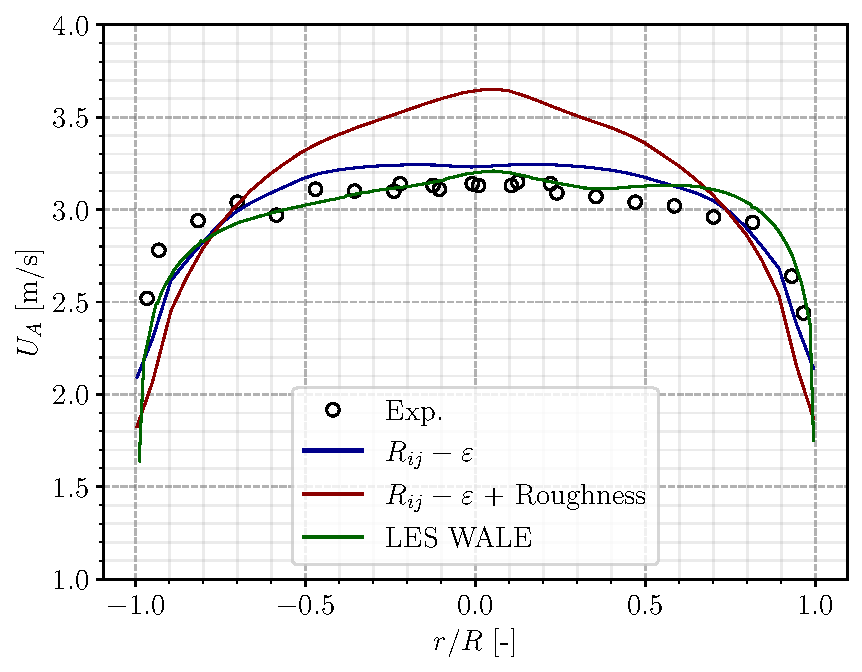
\includegraphics[width=0.4\linewidth]{img/AGATE/z440/pos910_VA.pdf}
\label{fig:agate_23dh_UA}
}
\subfloat[Radial velocity]{
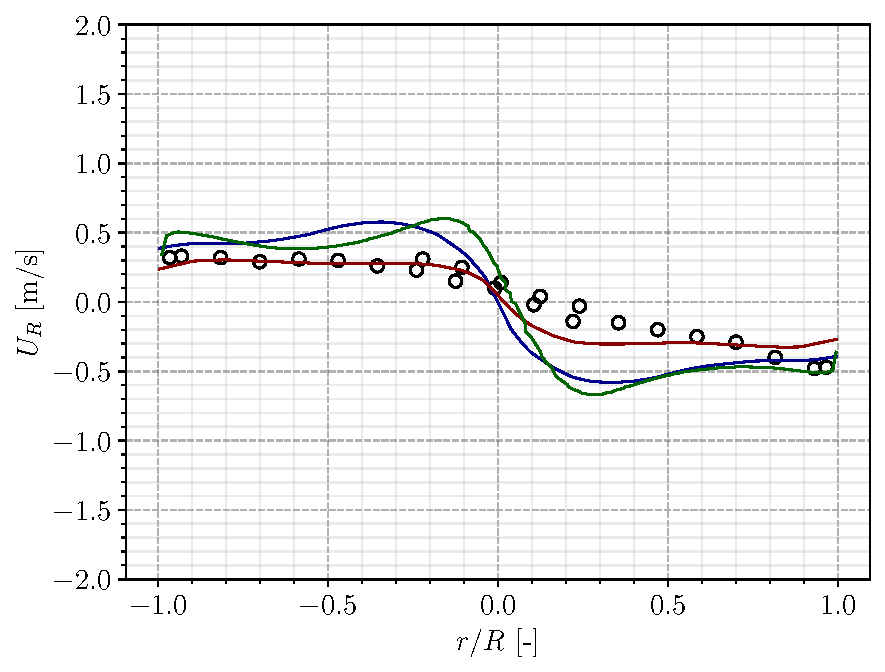
\includegraphics[width=0.4\linewidth]{img/AGATE/z440/pos910_VT.pdf}
\label{fig:agate_23dh_UR}
}
\\
\subfloat[Axial RMS]{
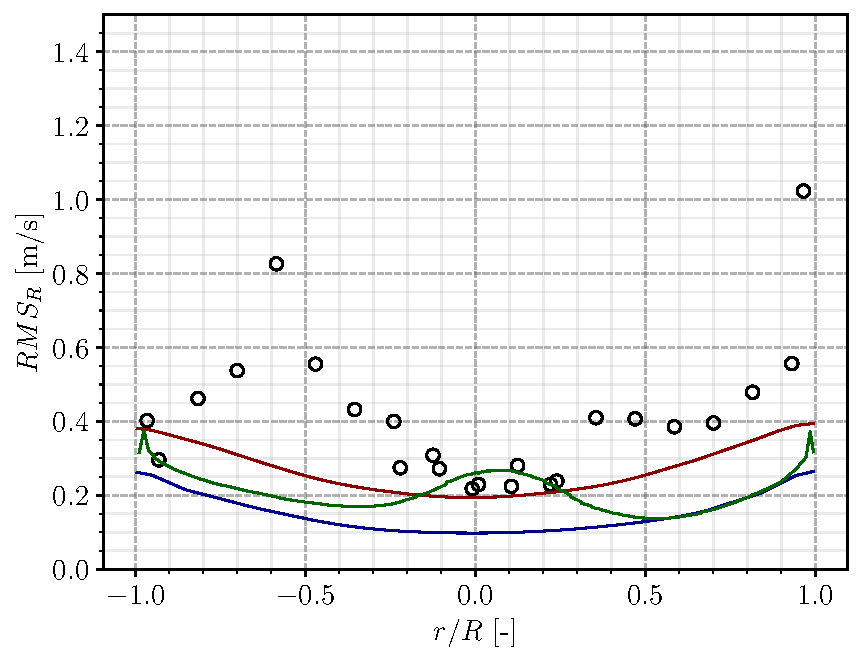
\includegraphics[width=0.4\linewidth]{img/AGATE/z440/pos910_RMS_A.pdf}
\label{fig:agate_23dh_RMSA}
}
\subfloat[Radial RMS]{
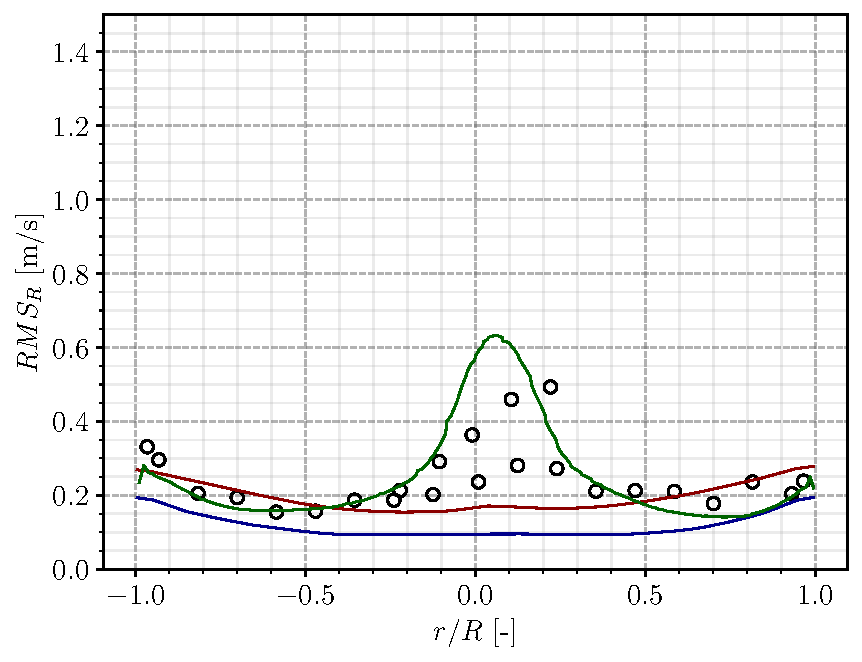
\includegraphics[width=0.4\linewidth]{img/AGATE/z440/pos910_RMS_T.pdf}
\label{fig:agate_23dh_RMSR}
}
\caption{Results for $z=22.9\ D_{h}$}
\label{fig:agate_cfd_23dh}
\end{figure}


\npar

At this distance, the axial velocity profile has been significantly degraded by using the roughness law (Figure\ \ref{fig:agate_23dh_UA}) where the other modelings continue to match the measurements. However, the overestimation of the rotation velocity is amplified compared to the $10\ D_{h}$ results for the smooth wall simulations while adding a roughness term seem to enhance the damping of the swirl induced by the vanes, better reproducing the experimental results (Figure \ref{fig:agate_23dh_UR}).

\npar

The axial velocity RMS are now better predicted by the rough wall simulation (Figure \ref{fig:agate_23dh_RMSA}) while the radial RMS is more accurately reproduced by the LES computation (Figure \ref{fig:agate_23dh_RMSR}). 


\npar

Figure \ref{fig:ur_s_ua_44dh} shows the ratio of radial to axial velocity $23~D_{h}$ after the vanes for the LES computation.

\begin{figure}
\subfloat[Instantaneous values]{
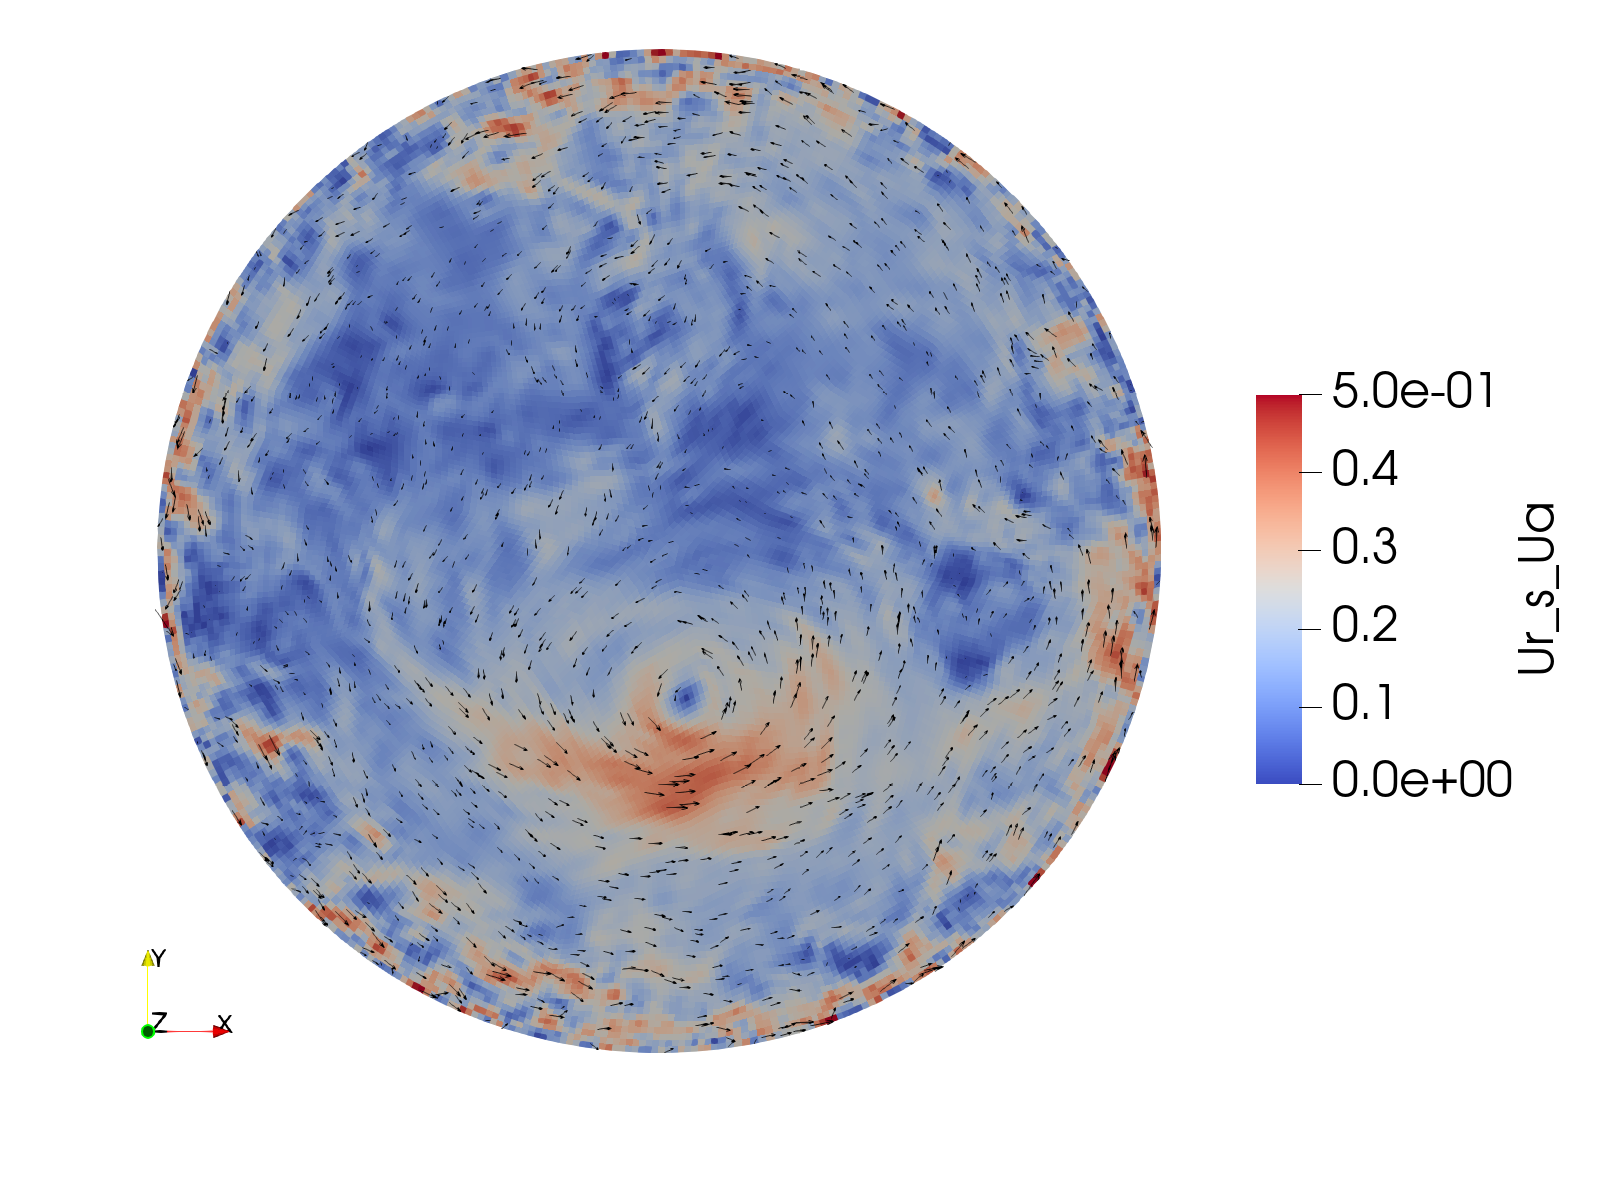
\includegraphics[width=0.5\linewidth]{img/AGATE/Ur_s_Ua/44Dh_Ur_s_Ua.png}
}
\subfloat[Time-averaged values]{
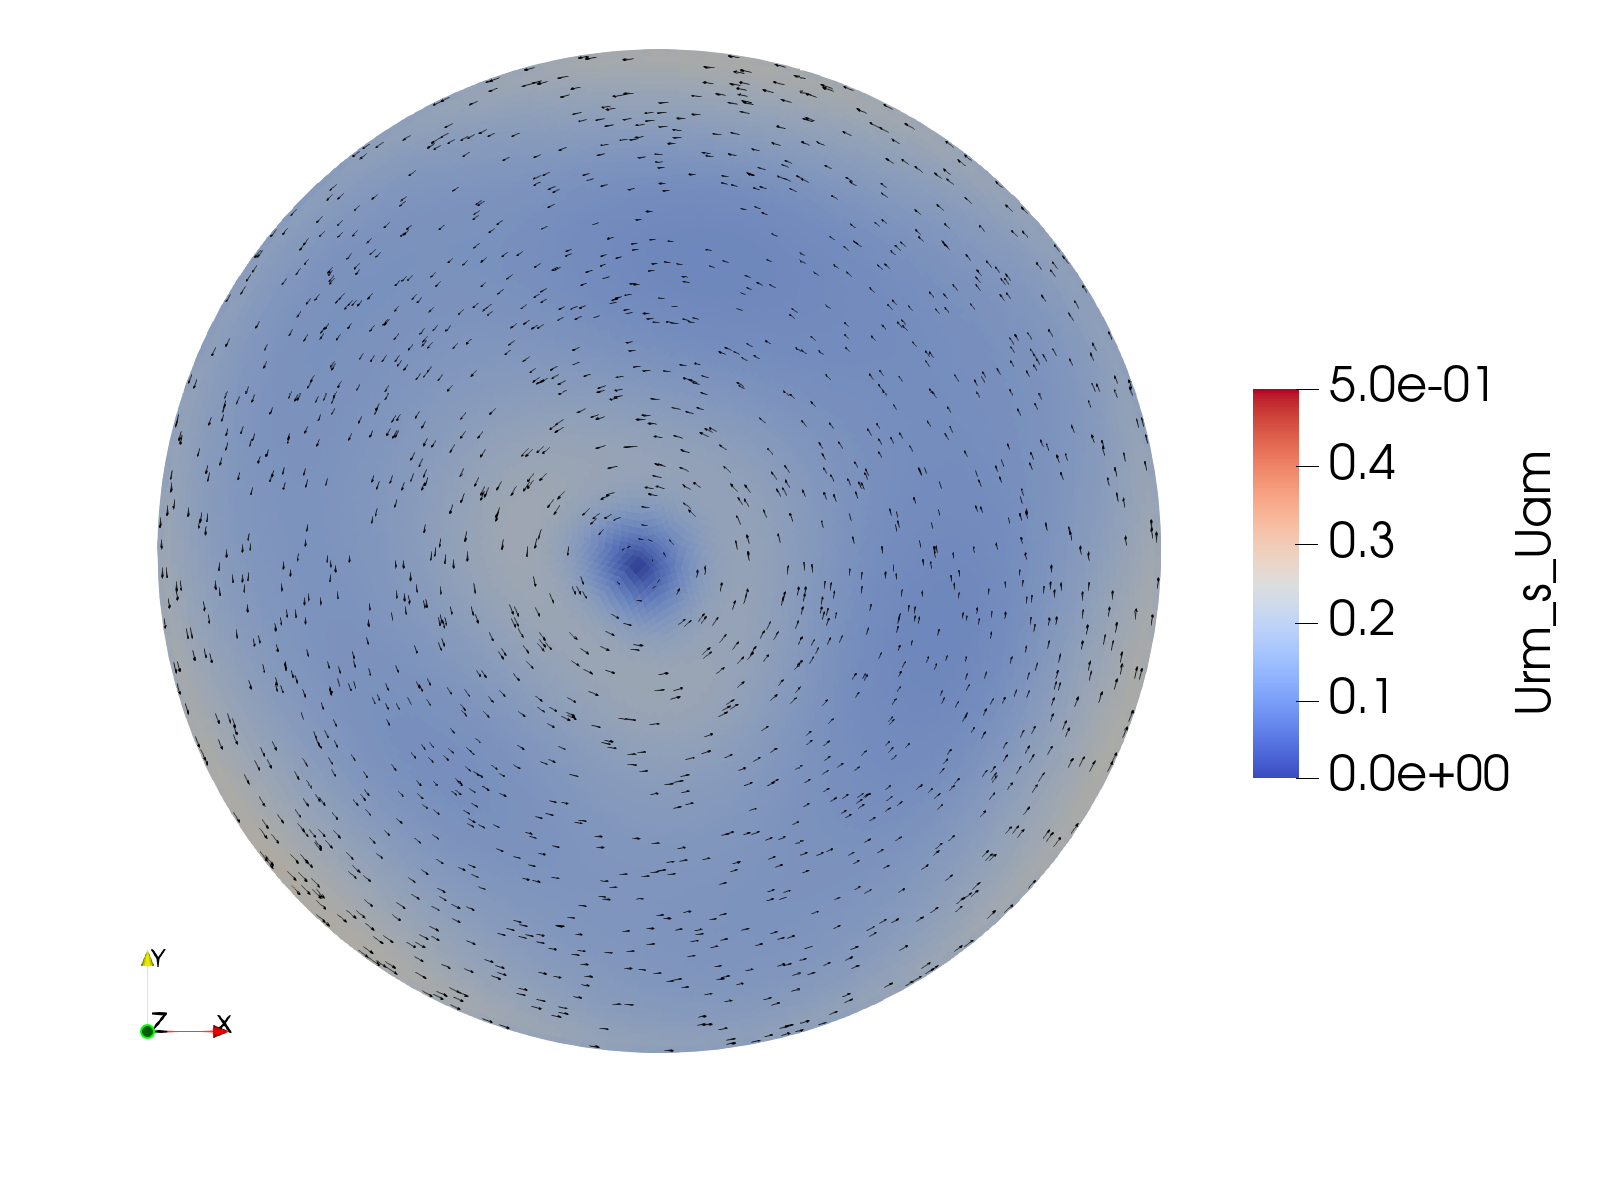
\includegraphics[width=0.5\linewidth]{img/AGATE/Ur_s_Ua/44Dh_Urm_s_Uam.png}
}
\caption{Visualization of the radial velocity field and ratio between radial and axial velocity obtained with the LES, $z=23~D_{h}$ downstream the MV.}
\label{fig:ur_s_ua_44dh}
\end{figure}



\clearpage



\subsubsection{Interpretation Regarding the DEBORA-Promoteur Simulations}

Overall, the main characteristic of the single-phase simulation results on the AGATE-Promoteur case is the overestimation of the radial velocity when moving downstream the mixing vanes and reaching the axial positions corresponding to C4800 and C5200 measurements. In terms of hydrodynamics, it means the fluid's rotation is too large, which will result in a stronger pressure gradient between the wall and the center. 

\npar

Transposing this result to a bubbly flow, the pressure gradient will be responsible for transverse migration of the bubbles towards the center of the pipe. If the rotation is overestimated, so will be the migration of bubbles which results in an excessive bubble accumulation in the core of the flow that should induce an overestimation of the local void fraction. This qualitative behavior is in agreement with the too large void fraction obtained in the simulations of DEBORA-Promoteur Te69 cases (Figure \ref{fig:debprom_ncfd}).

\npar

Moreover, the discrepancy on the rotation increasing with the distance to the mixing vanes implies that boiling simulations would be more accurate for the C5200 cases than the C4800 cases (measurements $10\ D_{h}$ downstream the MV versus. $23.5\ D_{h}$). That is actually true when looking at the void fraction profiles for Te65 and Te69 cases (Figures \ref{fig:Te65_cfd_alpha} and \ref{fig:Te69_cfd_alpha}) where larger differences with the measurements are observed for the C4800 simulations.



\begin{remark*}{}
The main limitation of the presented single-phase simulations is the systematic use of a wall-law, which can have a strong impact regarding this geometry where the wall presence is ubiquitous in addition to the mixing vanes presence. A LES computation using an even finer meshing allowing to reach $y^{+} \sim 1$ in the computational domain could bring insightful information to investigate the rotation overestimation.
\end{remark*}

%
%%
%\begin{figure}[!htb]
%\centering
%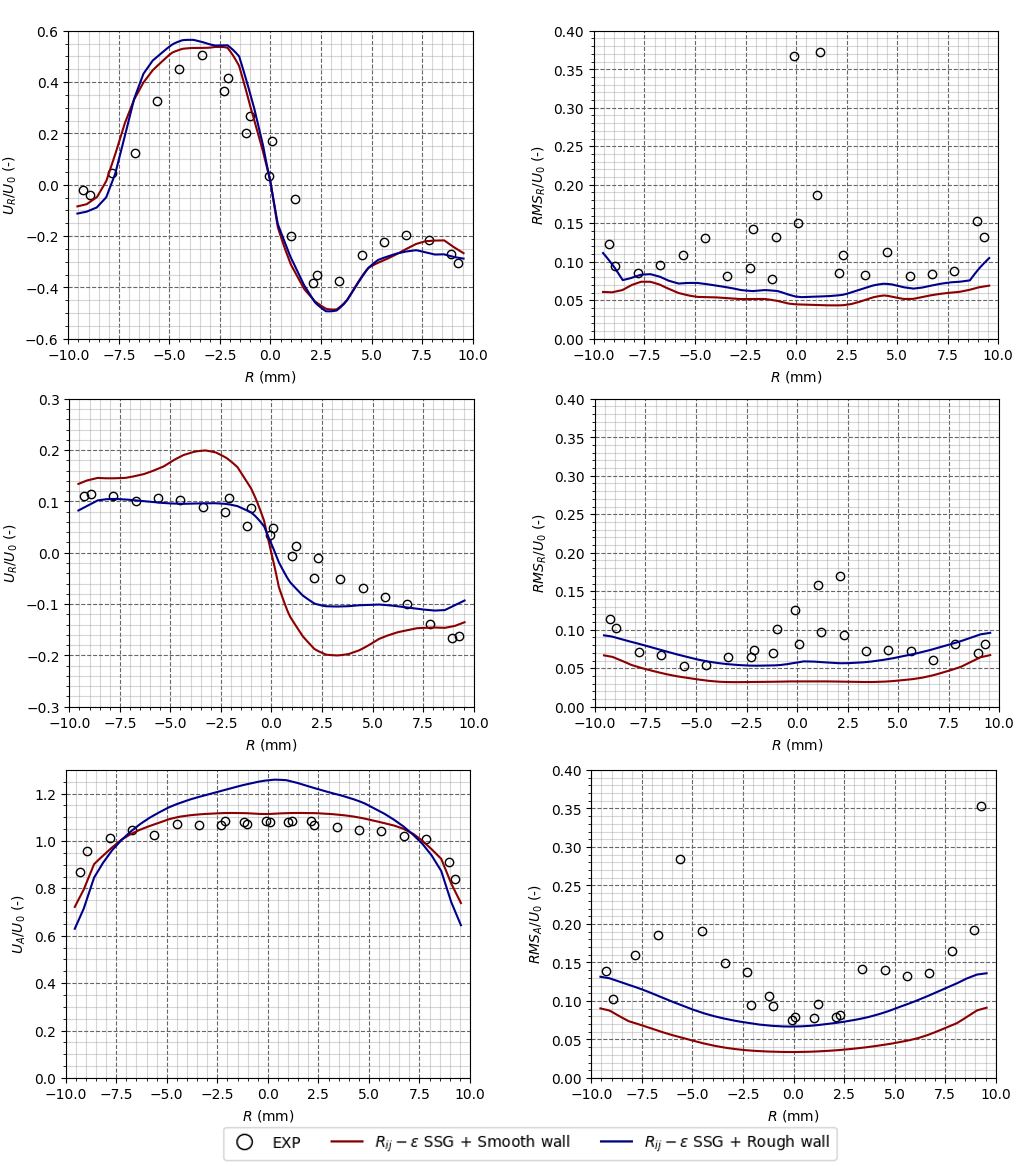
\includegraphics[scale=0.3]{img/AGATE/test.png}
%\caption{NCFD vs. Exp. - Top \& Middle : Radial velocity and turbulent RMS ($z=30$mm \& $z=440$mm) -  Bottom : Axial velocity and turbulent RMS ($z=440$mm).}
%\label{fig:agate1}
%\end{figure}
%
%Non-symmetric radial velocity profiles close to the MV are quite well reproduced by the simulations. However, far downstream the MV, it appears that the fluid's rotation is overestimated by the model with a smooth wall approach, while applying a roughness helps to reduce the magnitude of the swirl. Moreover, the radial turbulent fluctuations are better estimated by the rough wall approach at $z=440$~mm.
%
%On the other hand, it seems that the rough wall approach deteriorates the axial velocity profile compared to the experiment. As shown on the bottom part of Figure \ref{fig:agate1}, the smooth wall simulation returns a flat velocity profile closer to the experiment than the rough wall one which overestimates the core velocity peak.
%
%Both simulations globally underestimate the turbulent fluctuations, which can have a significant influence over the observed discrepancies on velocity profiles since turbulence plays a key role to homogenize the fluid flow. 
%
%Those results finally highlight the fact that simulation of such rotating flows may need a particular wall approach to better capture the induced swirl and its dissipation. Correct prediction of turbulent fluctuations would be of significant interest to ensure liquid velocity validation. Further investigations on boiling cases could possibly be improved by a roughness approach, which is the current correction used for two-phase wall laws (Subsection \ref{subsec:wall_func}). 


\section{Regarding CHF Detection in Mixing Vanes Geometry}

As a perspective test, we want to visualize the evolution of the CHF criterion of Zhang \cite{zhang_new_2022} (value of the CHF triplet $N_{sit,a} \pi \left<R\right>^{2} t_{g}f$), as in Section \ref{sec:chf_test_debora} on a DEBORA case, for a geometry including mixing vanes. To do so, a simulation of a boiling upward flow in a $5 \times 5$ heated rod bundle is conducted in PWR thermal-hydraulics conditions close to CHF. The geometry includes two PWR mixing grids and a non-uniform heating is applied with the 9 central rods having a larger wall heat flux. The initial NEPTUNE\_CFD Heat Flux Partitioning is used (Section \ref{sec:ncfd_HFP}) to compute the CHF triplet value.

\begin{note*}{}
As in Section \ref{sec:chf_test_debora}, the values of the CHF triplet attained in the computation are not in the range of [0,1] as it should be prior to CHF \cite{zhang_new_2022} since the closure laws for boiling parameters are not precise enough.
\end{note*}

On Figures \ref{fig:chf_grid1} and \ref{fig:chf_grid2} we present values obtained for the CHF triplet on the rods respectively at the first and the second grid. Wall areas where the CHF triplet is high are the zones closer to the boiling crisis.

\begin{figure}[!h]
\subfloat[Full rod bundle]{
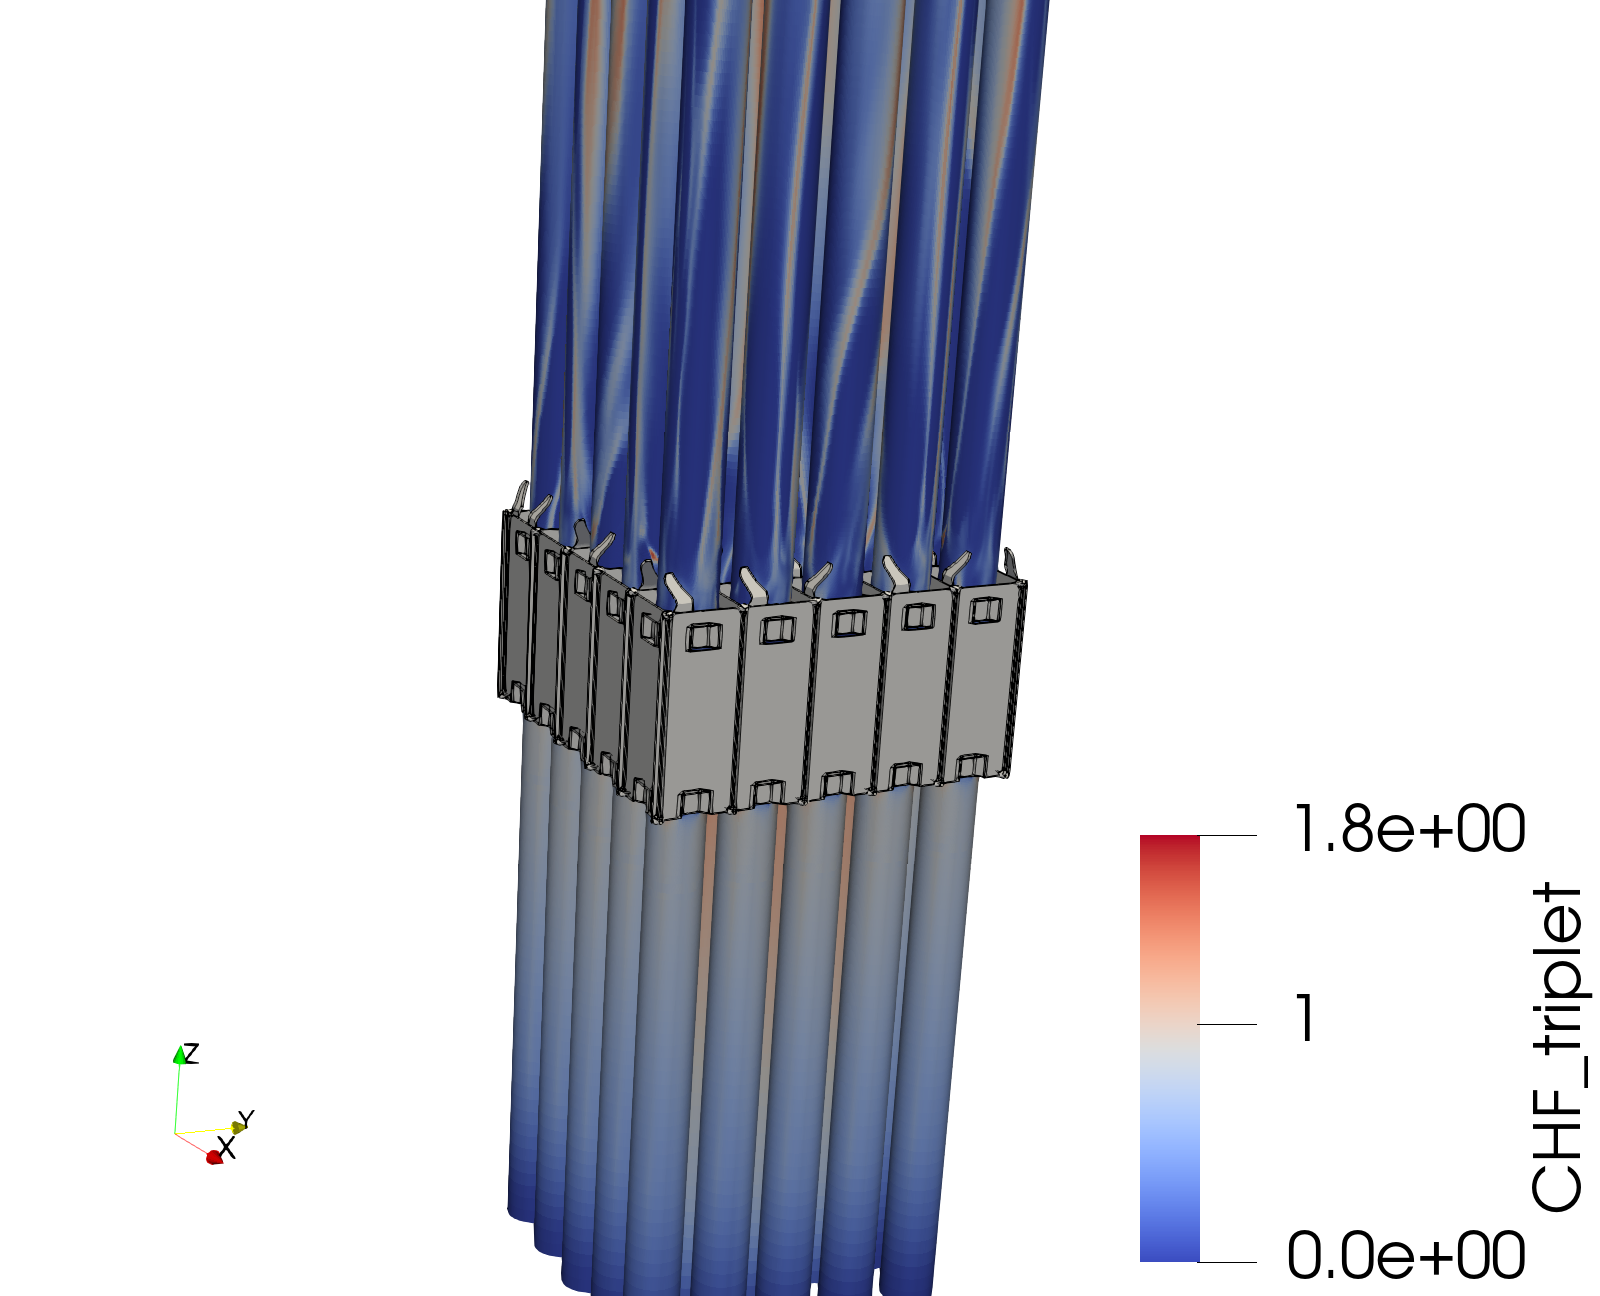
\includegraphics[width=0.5\linewidth]{img/chf/chf_crit/grid1_full.png}
}
\subfloat[Clip of the bundle, showing the central rods]{
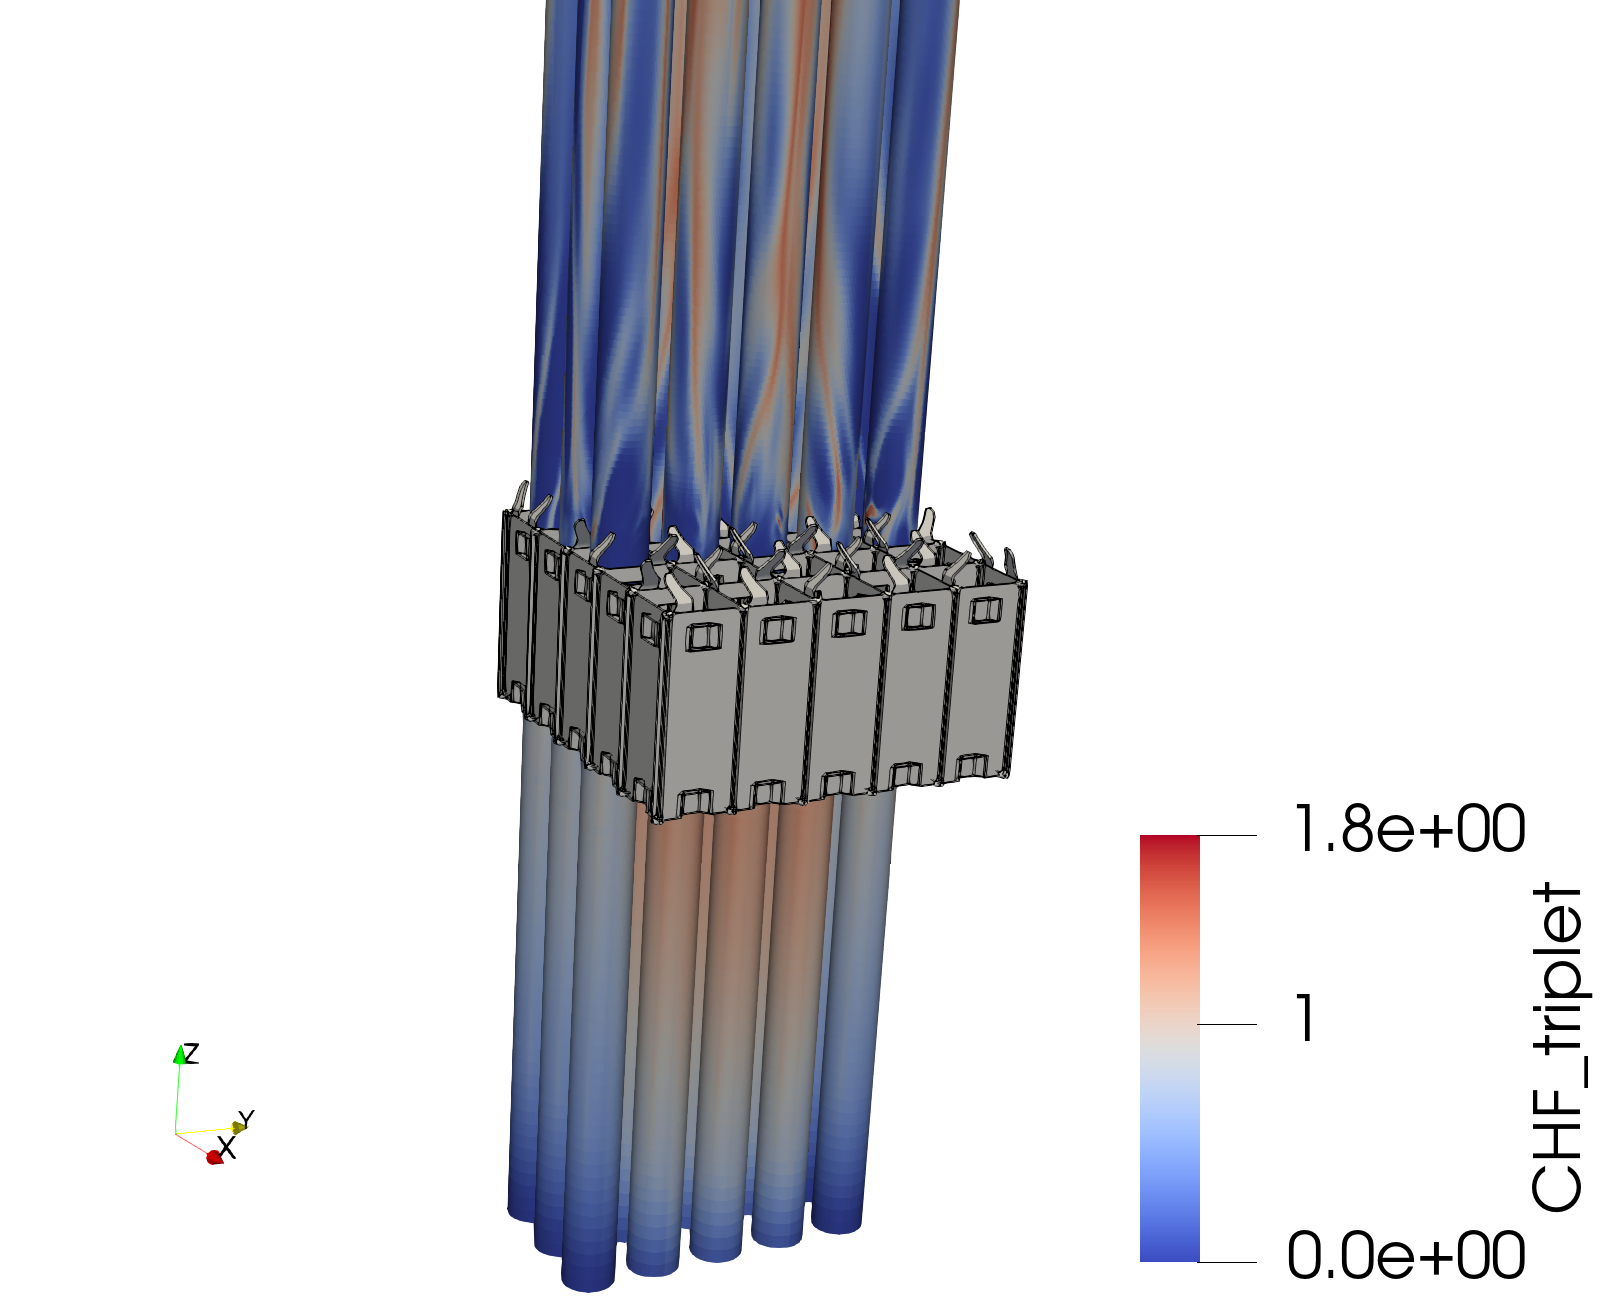
\includegraphics[width=0.5\linewidth]{img/chf/chf_crit/grid1.png}
}
\caption{Visualization of the CHF triplet value around the first grid. (Computation results courtesy of Vladimir Duffal)}
\label{fig:chf_grid1}
\end{figure} 


\begin{figure}[!h]
\subfloat[Full rod bundle]{
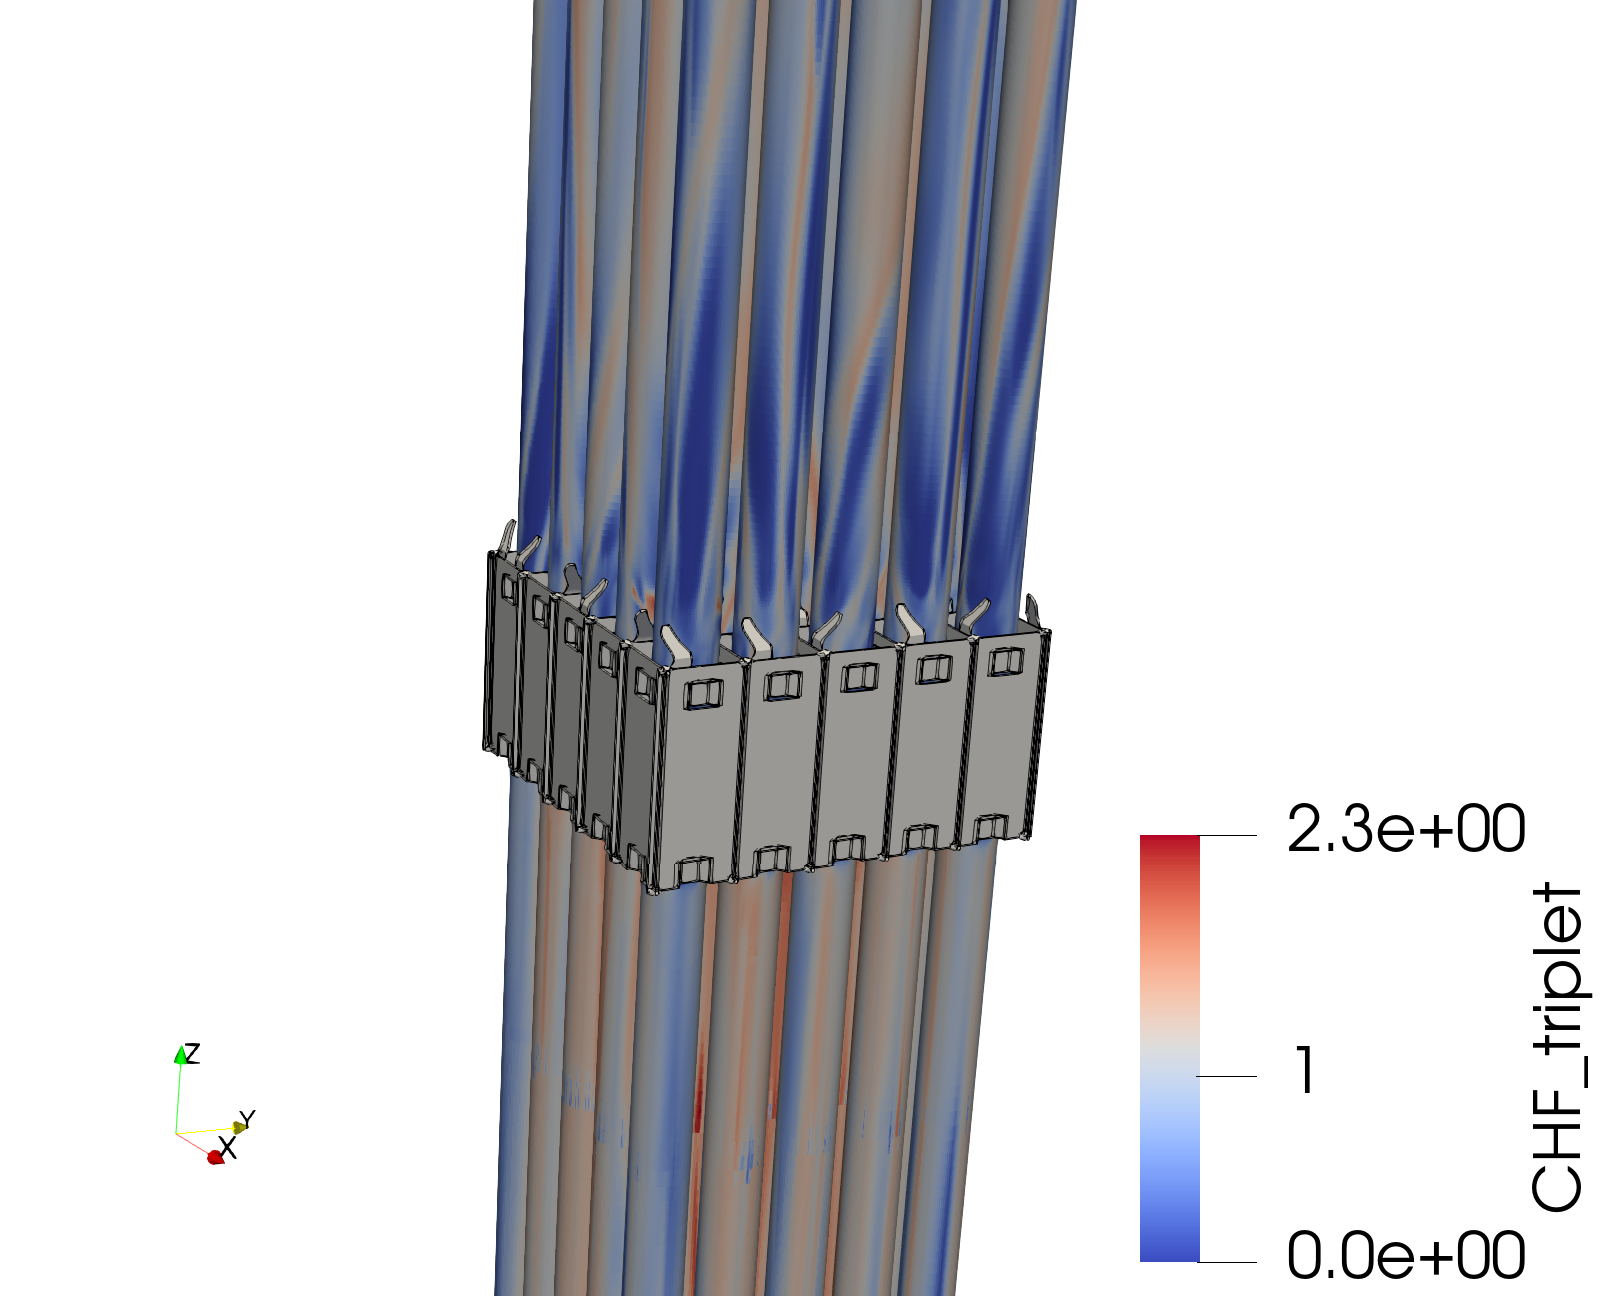
\includegraphics[width=0.5\linewidth]{img/chf/chf_crit/grid2_full.png}
}
\subfloat[Clip of the bundle, showing the central rods]{
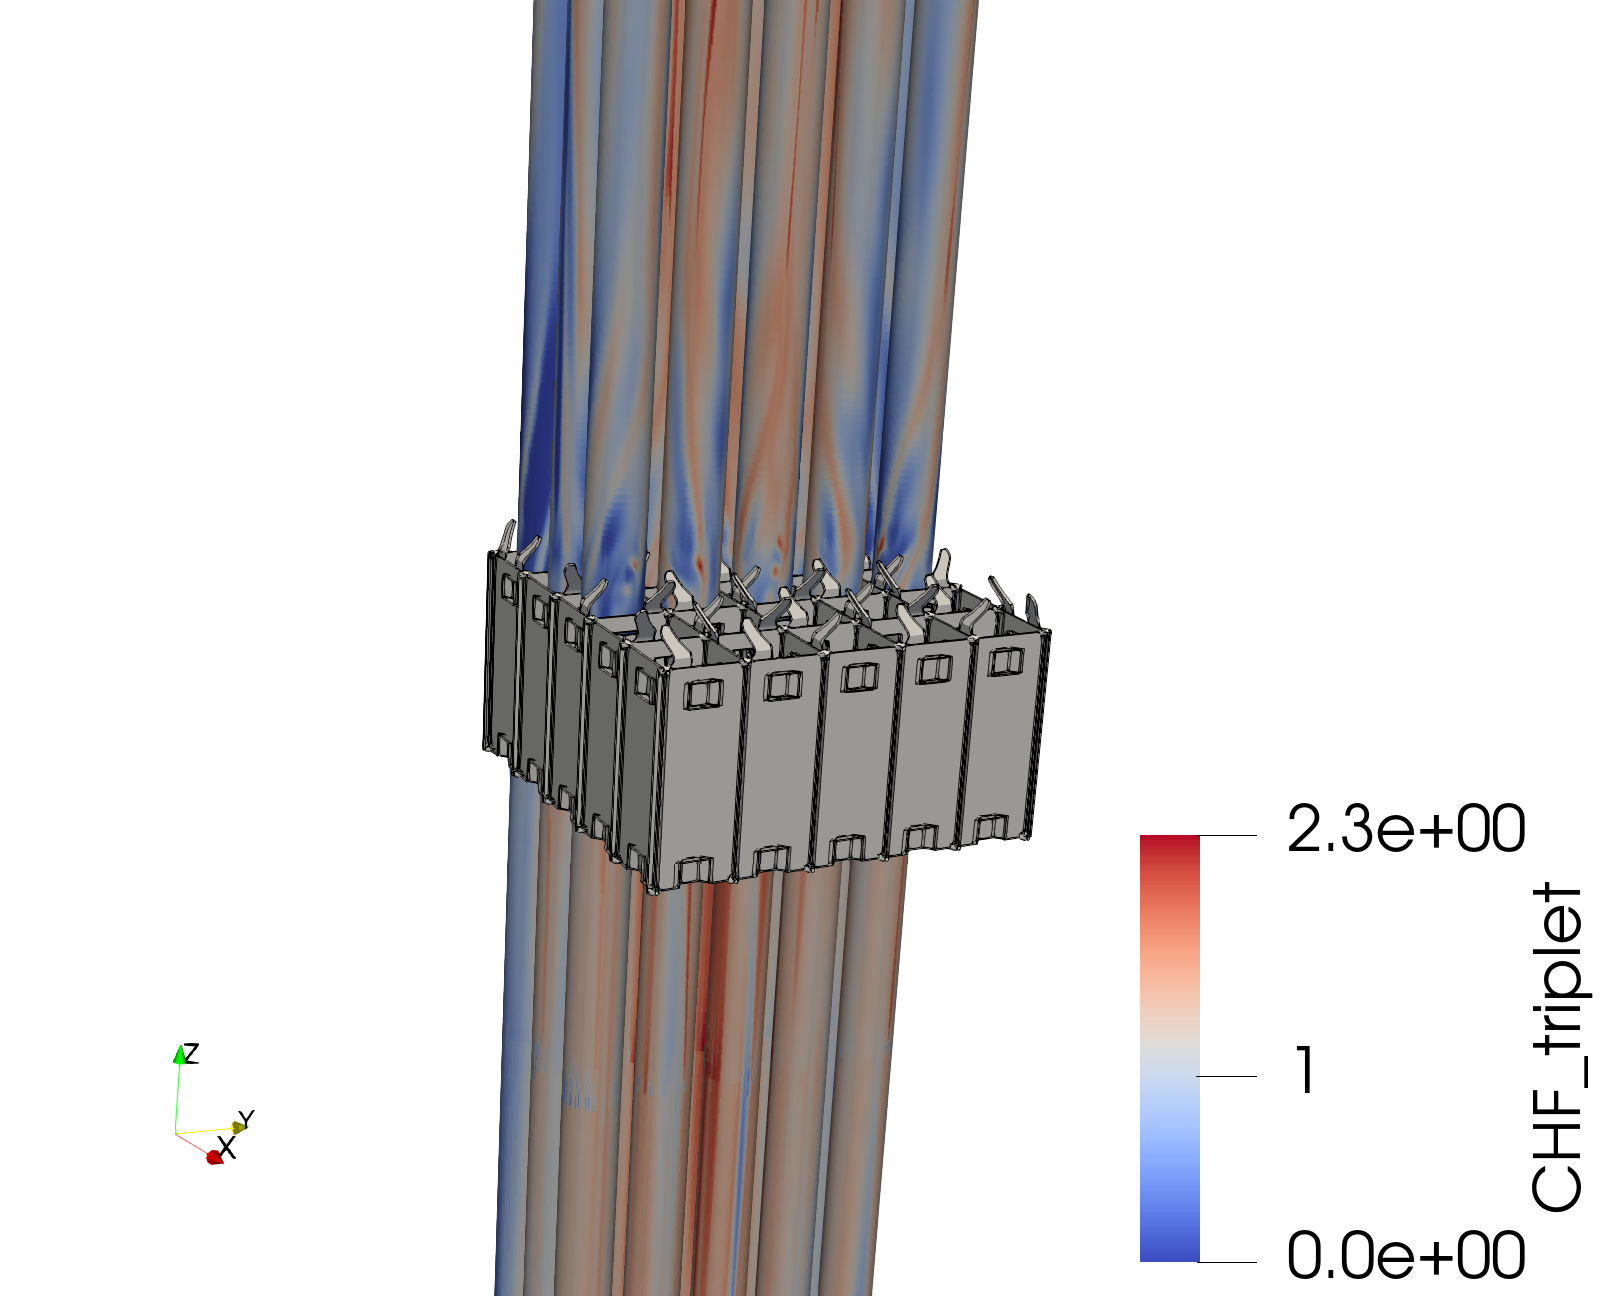
\includegraphics[width=0.5\linewidth]{img/chf/chf_crit/grid2.png}
}
\caption{Visualization of the CHF triplet value around the second grid. (Computation results courtesy of Vladimir Duffal)}
\label{fig:chf_grid2}
\end{figure}

\npar
At the inlet upwards the first mixing vane (Figure \ref{fig:chf_grid1}), the CHF triplet gradually increases similar to a simple tube case (Figure \ref{fig:debora_chf_criterion}) with the central rods exposed to a larger heat flux reaching greater values of the CHF triplet. After the vanes, the local values of the CHF criterion are significantly diminished both for peripheral and central rods, with non-symmetric patterns related to the rotating flow induced by the mixing vanes.



\npar 
When reaching the second grid (Figure \ref{fig:chf_grid2}), the difference in CHF triplet values between central and peripheral rods is less important which is probably an effect of the upwards mixing of the first grid. After the second grid, the CHF triplet values are also globally reduced similar to what was observed at the first grid (Figure \ref{fig:chf_grid1}). The CHF triplet is though larger when reaching the second grid, which is logical since the fluid is continuously heated between the two grids. Higher risk of boiling crisis would seem to be right upstream the second grid.

\npar

Altogether, those observations, though purely qualitative, are presenting interestingly coherent features regarding boiling crisis occurrence for PWR with overheated rods have larger CHF triplet values and mixing grids actually decrease the CHF triplet thanks to their mixing effect.

\clearpage


\section{Conclusions}

In this Chapter, we performed CFD simulations on the tube equipped with mixing vanes geometry. Both boiling flow simulations using NEPTUNE\_CFD and single-phase simulations with \textit{code\_saturne} were realized, respectively compared to DEBORA-Promoteur and AGATE-Promoteur experiments. So far, the main highlights of the results are:

\begin{itemize}
\item The boiling simulations of DEBORA-Promoteur cases showed reasonable qualitative behavior with bulk vapor accumulation, void fraction peak and bubble coalescence at the center, and vapor velocity increase with outlet quality.

\item Yet, precise predictions of void fraction profiles could not be achieved with very large overestimation in the bulk plus the incapacity to reach void fractions higher than 70\%. This could be associated to change in the multiphase flow regime that lie outside of the dispersed bubbly flow model capacity.

\item Further investigations on the single phase case AGATE-Promoteur showed an excessive computed rotation of the fluid, increasingly differing from the experiments as we move downstream the mixing vanes. A too large swirl could explain the overestimation of the void fraction in the boiling case due to bubble transverse migration.

\item Wall law seems to have a significant influence over the velocity profiles and may be an area of improvement, especially for confined geometries where solid walls are strongly influencing the flow.

\begin{remark*}{}
We want to mention that achieving precise results for single-phase simulations on complex industrial geometries representative of PWR is still a very active field of research \cite{lee_synthesis_2014}. The use of RANS \cite{benhamadouche_use_2017} or wall-modeled LES \cite{gauffre_wall-modeled_2020} approaches are still investigated in order to save computational time in the prospect of reaching simulations of a full fuel assembly by including, for instance, modeling of mixing vanes as source terms in the computational domain \cite{capone_source_2016}.
\end{remark*}

\item Evaluating values of the CHF triplet as a qualitative indicator of boiling crisis risk of occurrence (Section \ref{sec:chf_test_debora}) on a rod bundle including mixing vanes showed presented a good perspective with physically coherent evolution regarding the overheated rods and mixing grids effects. This could be compared to boiling crisis location in experiments to further validate its behavior.
\end{itemize}


%\section{Towards Prediction of the Critical Heat Flux in Industrial Geometries ?}